\documentclass[conference,letterpaper]{IEEEtran}
\IEEEoverridecommandlockouts
\usepackage[utf8]{inputenc}
\usepackage[T1]{fontenc}
\usepackage[spanish,es-nodecimaldot,es-noshorthands]{babel}
\usepackage{amsmath,amssymb}
\usepackage{graphicx}
\usepackage{booktabs}
\usepackage{array}
\usepackage{url}
\usepackage{xcolor}
\usepackage{cite}
\usepackage{placeins}
\addto\captionsspanish{\renewcommand{\figurename}{Fig.}\renewcommand{\tablename}{TABLA}}

\graphicspath{{figs/}}
\renewcommand{\topfraction}{0.9}\renewcommand{\bottomfraction}{0.6}
\renewcommand{\textfraction}{0.08}\renewcommand{\floatpagefraction}{0.75}
\renewcommand{\dbltopfraction}{0.9}\renewcommand{\dblfloatpagefraction}{0.75}
\setcounter{topnumber}{3}\setcounter{dbltopnumber}{2}\setcounter{totalnumber}{5}
\newcommand{\Hhat}{\hat{H}}
\newcommand{\bhat}{\hat{\beta}}

\begin{document}

\title{Autosimilitud en trazas de tráfico LAN: estimación del parámetro de Hurst por varianza agregada en una red emulada}

\author{\IEEEauthorblockN{Ivan Camilo Cometa}
\IEEEauthorblockA{Programa de Ciencias de la Computación\\ e Inteligencia Artificial\\
Universidad Sergio Arboleda\\
Bogotá D.C., Colombia}
\and
\IEEEauthorblockN{Francisco Morales}
\IEEEauthorblockA{Programa de Ciencias de la Computación\\ e Inteligencia Artificial\\
Universidad Sergio Arboleda\\
Bogotá D.C., Colombia}}

\maketitle

\begin{abstract}
Se estudió si el tráfico UDP de una LAN de tres nodos presenta autosimilitud de segundo orden. La red se emuló con \emph{network namespaces} de Linux y un \emph{bridge} como switch, y se capturaron cuatro corridas de 600~s con iperf3 y tcpdump: dos con tasa constante (E1) y dos con ráfagas intermitentes de dos fuentes (E2). Cada traza se convirtió en una serie de bytes por intervalo ($\Delta = 0.05$~s) y se estimó $H$ por el método de varianza agregada, con selección objetiva del tramo lineal, control por 30 permutaciones, repetición con $\Delta = 0.10$~s y periodograma. E1 resultó antipersistente ($\Hhat = 0.03$--$0.05$, pendiente $\approx -1.9$) frente a un control de $0.49$--$0.51$, con un ciclo de 0.3~s atribuible al muestreo. E2 dio $\Hhat = 0.97$--$0.98$ entre 0.05 y 3.2~s, muy por encima del control, pero su pendiente local cambia de $0$ a $-0.9$ hacia 12.8~s: es la huella del cronograma ON/OFF de 1--20~s y no un escalamiento autosimilar. Las conclusiones se repiten entre corridas y resoluciones ($|\Delta\Hhat| \le 0.024$).
\end{abstract}

\begin{IEEEkeywords}
autosimilitud, parámetro de Hurst, varianza agregada, tráfico LAN, iperf3, prueba de permutación.
\end{IEEEkeywords}

\section{Introducción}
Leland \emph{et al.}~\cite{leland94} mostraron que el tráfico Ethernet real es estadísticamente autosimilar: sus ráfagas no se suavizan al agregarlo en escalas de tiempo crecientes, a diferencia de los modelos de Poisson. Este comportamiento se ha explicado como la superposición de muchas fuentes ON/OFF con periodos de alta variabilidad~\cite{willinger97}. El objetivo de este trabajo es medir si el tráfico generado en dos escenarios controlados es compatible con autosimilitud de segundo orden y en qué escalas, distinguiendo un escalamiento real de uno aparente producido por pausas programadas o por la duración finita de la captura.

\begin{figure*}[!t]
\centering
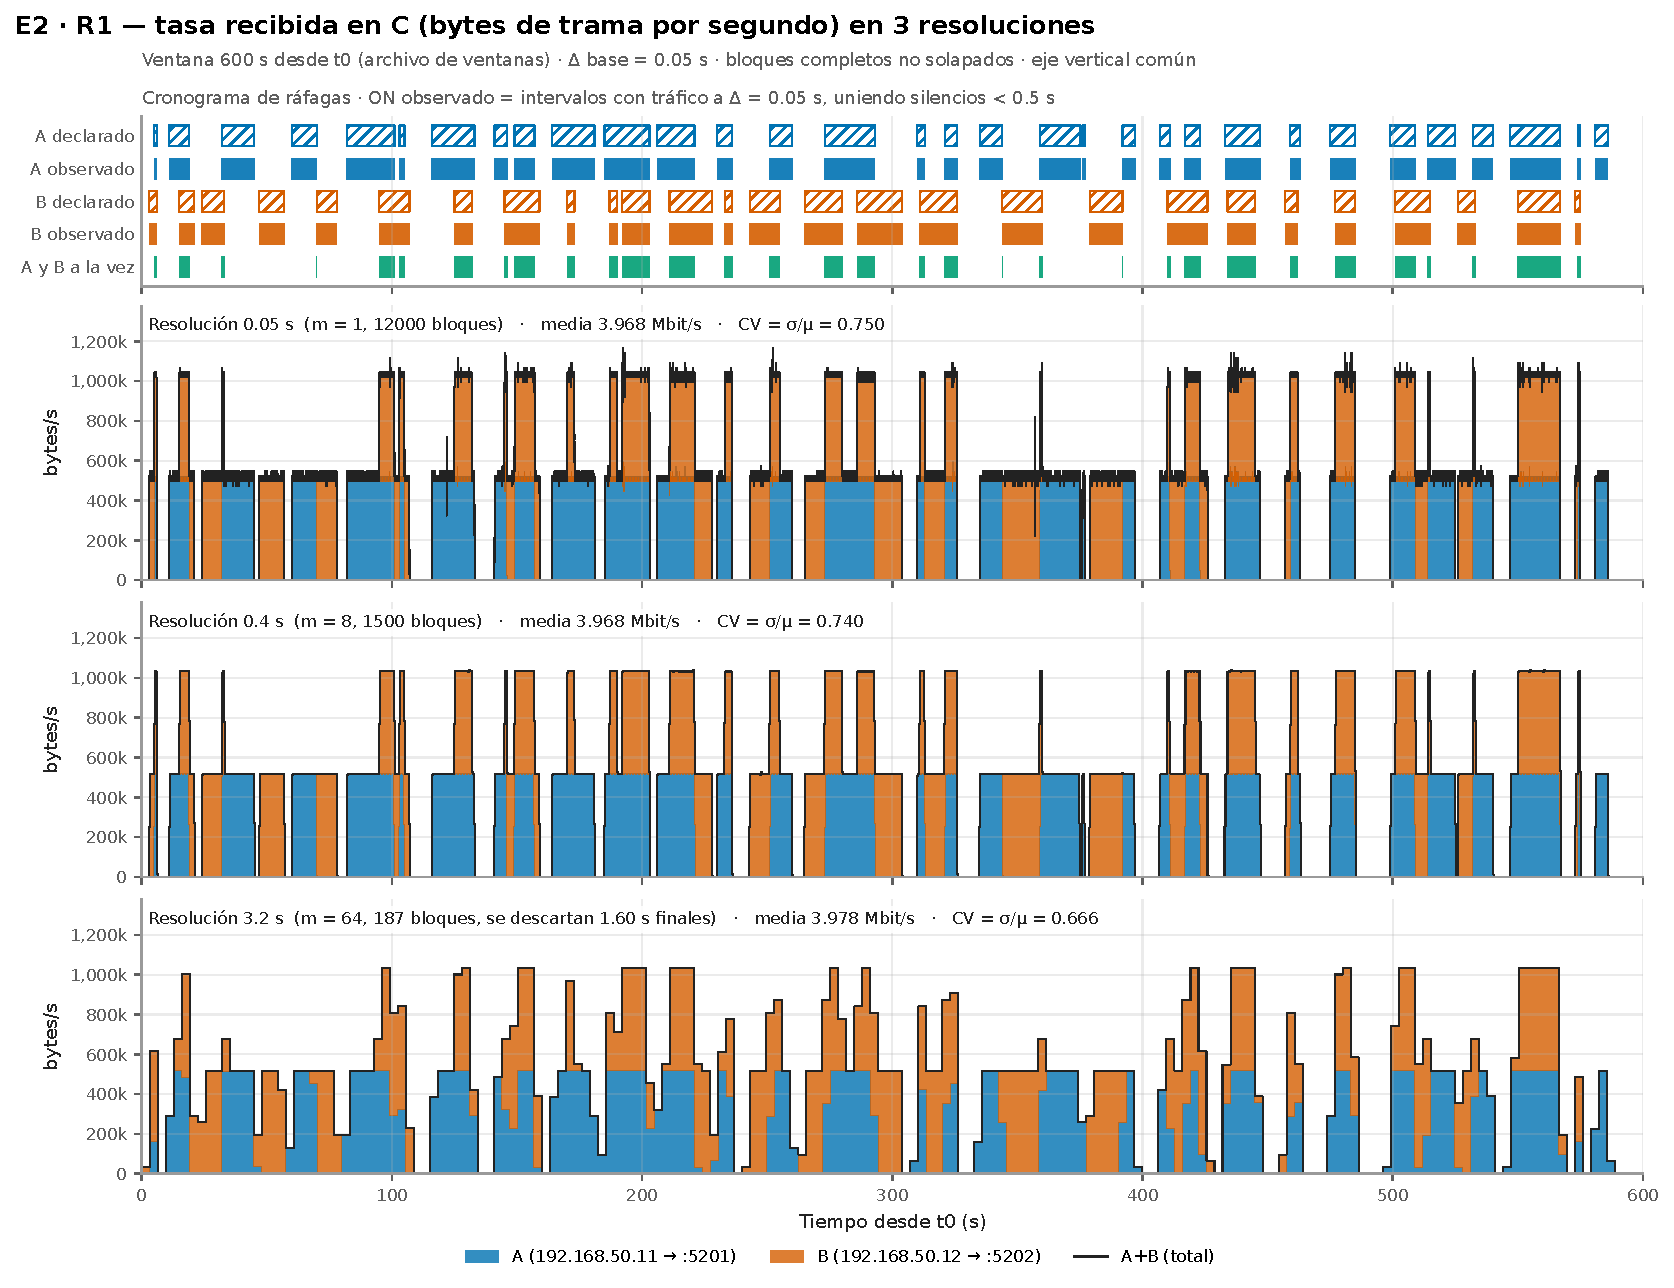
\includegraphics[width=0.92\textwidth]{ts_E2_R1.pdf}
\caption{E2\_R1: tasa recibida en C a 0.05, 0.4 y 3.2~s (A y B apiladas; el borde superior es A+B) y franja con el cronograma declarado y las ráfagas observadas.}
\label{fig:ts}
\end{figure*}

\section{Montaje experimental}
\subsection{Topología}
Por no disponer de tres equipos físicos, la LAN se emuló en un anfitrión Linux (Ubuntu 24.04.5, kernel 6.18, 2 núcleos). Cada nodo es un \emph{network namespace} y el switch un \emph{bridge} de Linux, el mismo mecanismo que usa Mininet~\cite{lantz10}. Los enlaces son pares \emph{veth} sin limitación de tasa. La Tabla~\ref{tab:nodos} resume la configuración y la Fig.~\ref{fig:red} la topología. Antes de cada corrida, 5 \texttt{ping} de A y B hacia C dieron 0\,\% de pérdida y un RTT medio de 0.05--0.06~ms.

\begin{table}[!t]
\caption{Nodos de la red emulada}
\label{tab:nodos}
\centering
\footnotesize
\setlength{\tabcolsep}{3pt}
\begin{tabular}{@{}llll@{}}
\toprule
Nodo & Rol & IP & Interfaz \\
\midrule
A & Cliente iperf3, puerto 5201 & 192.168.50.11/24 & eth0 (veth)\\
B & Cliente iperf3, puerto 5202 & 192.168.50.12/24 & eth0 (veth)\\
C & Servidor iperf3 y captura & 192.168.50.13/24 & eth0 (veth)\\
Switch & \emph{bridge} de Linux & --- & un puerto por nodo\\
\bottomrule
\end{tabular}\\[2pt]
\raggedright\scriptsize Software: iperf3 3.16, tcpdump 4.99.4, TShark 4.2.2.
\end{table}

\begin{figure}[!t]
\centering
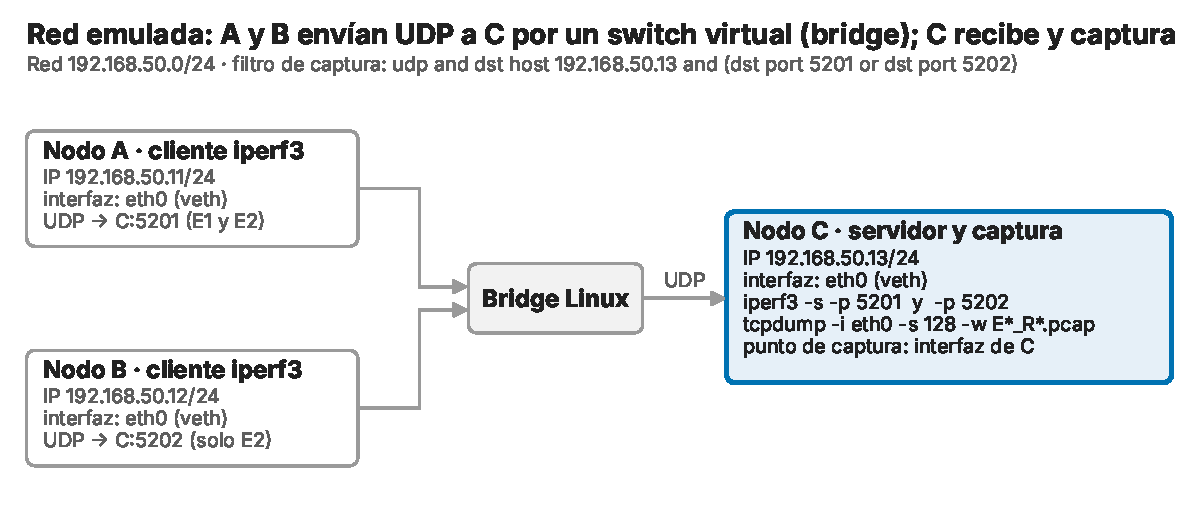
\includegraphics[width=\columnwidth]{diagrama_red.pdf}
\caption{Topología emulada: A y B envían UDP a C a través del \emph{bridge}; C captura en su interfaz.}
\label{fig:red}
\end{figure}

\subsection{Escenarios}
\textbf{E1} (tasa constante): A envía a C:5201 con \texttt{iperf3 -u -b 4M -l 1200 -t 600}; la ventana empieza en el primer datagrama recibido. \textbf{E2} (intermitente): A (puerto 5201) y B (puerto 5202) siguen cronogramas distintos, sorteados con semilla fija, con silencio inicial de 2--6~s, ráfagas y pausas de 1--20~s y silencio final $\ge 8$~s; la ventana fija de 600~s empieza 0.5~s antes de la primera ráfaga. Se hicieron dos repeticiones de cada escenario. E1\_R1 y E1\_R2 se ejecutaron en paralelo en redes aisladas (un emisor cada una) y las de E2 por separado, de modo que nunca hubo más emisores que núcleos.

\subsection{Adquisición}
En C se capturó con \texttt{tcpdump -i eth0 -nn -s 128} y el filtro \texttt{udp and dst host 192.168.50.13 and (dst port 5201 or dst port 5202)}, y se exportó con TShark los campos \texttt{frame.time\_epoch}, \texttt{frame.len}, \texttt{ip.src} y \texttt{udp.dstport}. La Tabla~\ref{tab:corridas} registra las ventanas, las pérdidas UDP reportadas por iperf3 y los descartes del capturador.

\begin{table}[!t]
\caption{Registro de corridas (reloj de C, epoch)}
\label{tab:corridas}
\centering
\scriptsize
\setlength{\tabcolsep}{3pt}
\begin{tabular}{@{}lllll@{}}
\toprule
Corrida & $t_0$ & Fin captura & Pérdida UDP & Desc.\\
\midrule
E1\_R1 & 1795062526.7116 & 1795063129.7226 & 0/250\,000 & 0\\
E1\_R2 & 1795062528.7189 & 1795063131.7334 & 0/250\,000 & 0\\
E2\_R1 & 1795063137.8008 & 1795063742.8009 & A 0/125\,001; B 0/114\,582 & 0\\
E2\_R2 & 1795063748.8853 & 1795064353.8855 & A 0/112\,499; B 0/117\,085 & 0\\
\bottomrule
\end{tabular}
\end{table}

\begin{figure*}[!t]
\centering
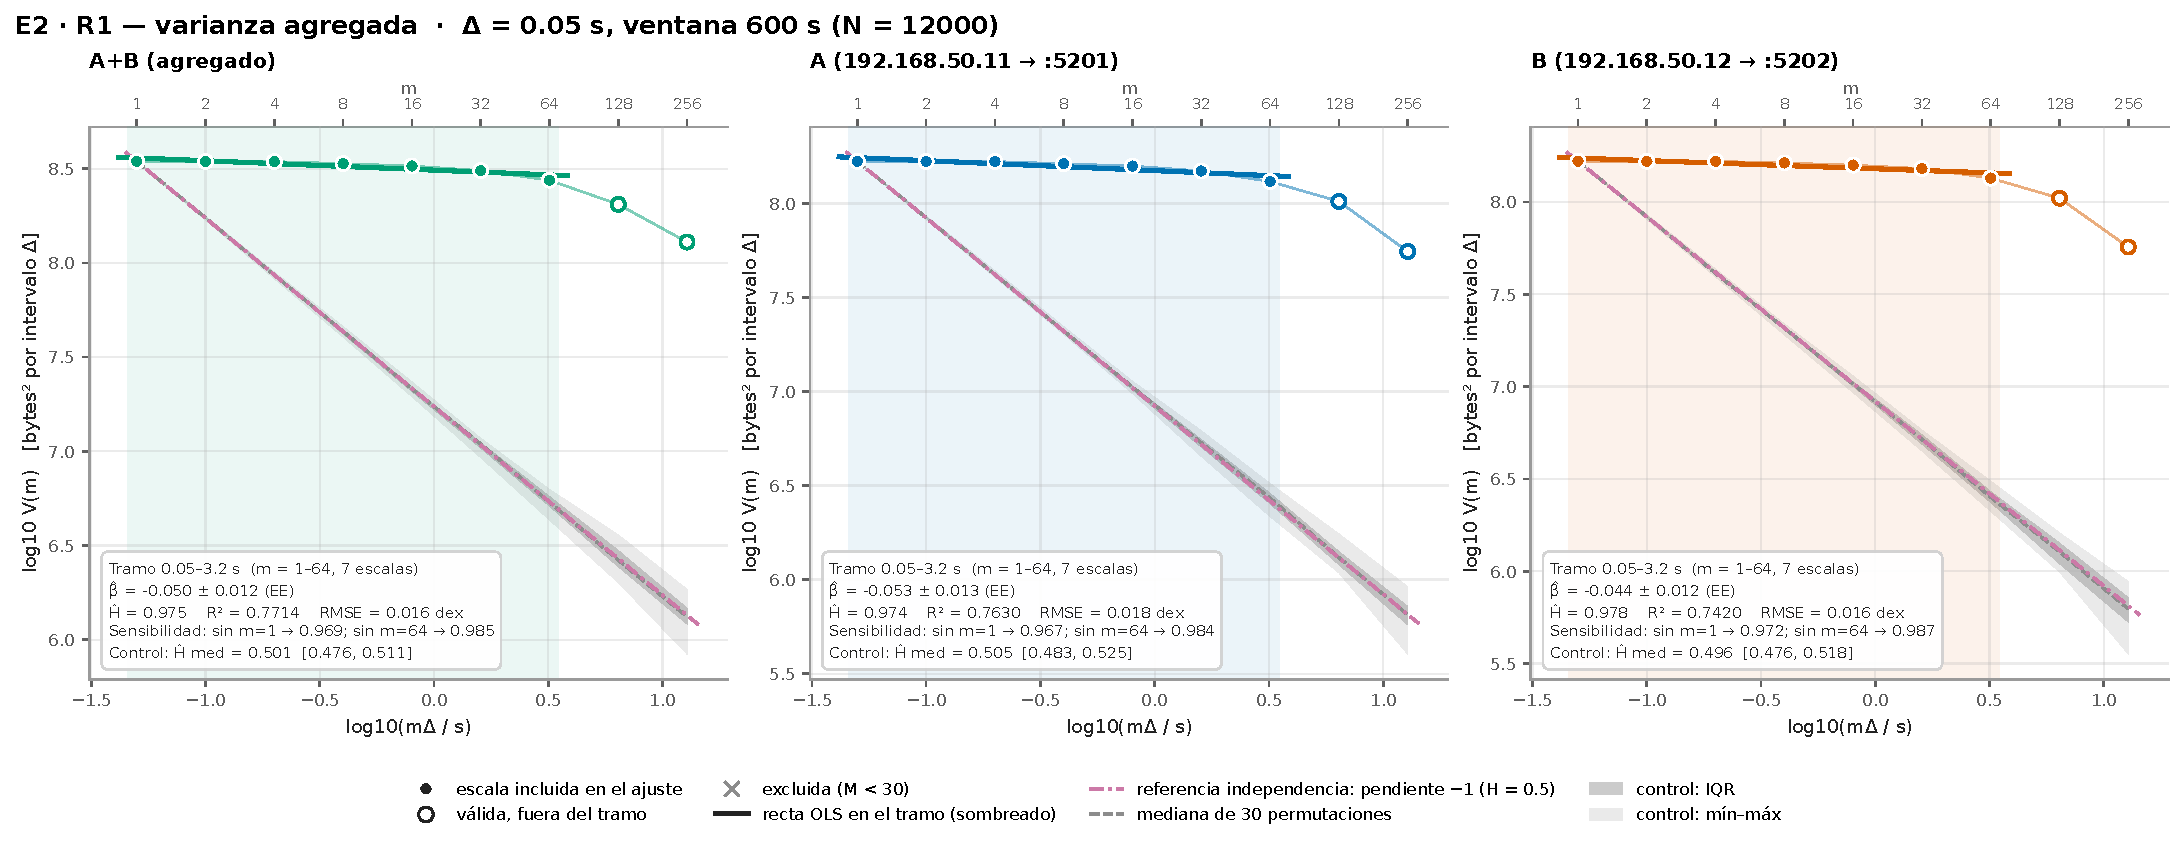
\includegraphics[width=\textwidth]{vt_E2_R1_d005.pdf}
\caption{E2\_R1: varianza agregada de A+B, A y B ($\Delta = 0.05$~s) frente al control permutado.}
\label{fig:vte2}
\end{figure*}

\begin{table*}[!t]
\caption{Resultados por corrida, serie y resolución (pérdida UDP y descartes de captura: 0 en todas)}
\label{tab:res}
\centering
\footnotesize
\begin{tabular}{@{}cccccccccc@{}}
\toprule
Esc. & Rep. & Serie & $\Delta$ (s) & Tramo (s) & $\bhat$ & $\Hhat$ & $R^2$ & $\Hhat$ control: mediana [mín, máx] & $\Hhat$ frente al control\\
\midrule
E1 & R1 & A & 0.05 & 1.6--12.8 & $-1.894$ & 0.053 & 0.999 & 0.509 [0.397, 0.577] & por debajo\\
E1 & R1 & A & 0.10 & 1.6--12.8 & $-1.894$ & 0.053 & 0.999 & 0.493 [0.387, 0.562] & por debajo\\
E1 & R2 & A & 0.05 & 0.1--0.8 & $-1.941$ & 0.029 & 0.999 & 0.494 [0.481, 0.526] & por debajo\\
E1 & R2 & A & 0.10 & 0.1--0.8 & $-1.941$ & 0.029 & 0.999 & 0.502 [0.486, 0.521] & por debajo\\
\midrule
E2 & R1 & A+B & 0.05 & 0.05--3.2 & $-0.050$ & 0.975 & 0.771 & 0.501 [0.476, 0.511] & por encima\\
E2 & R1 & A & 0.05 & 0.05--3.2 & $-0.053$ & 0.974 & 0.763 & 0.505 [0.483, 0.525] & por encima\\
E2 & R1 & B & 0.05 & 0.05--3.2 & $-0.044$ & 0.978 & 0.742 & 0.496 [0.476, 0.518] & por encima\\
E2 & R1 & A+B & 0.10 & 0.1--3.2 & $-0.062$ & 0.969 & 0.832 & 0.503 [0.478, 0.525] & por encima\\
E2 & R1 & A & 0.10 & 0.1--3.2 & $-0.066$ & 0.967 & 0.824 & 0.499 [0.470, 0.529] & por encima\\
E2 & R1 & B & 0.10 & 0.1--3.2 & $-0.056$ & 0.972 & 0.801 & 0.503 [0.463, 0.534] & por encima\\
E2 & R2 & A+B & 0.05 & 0.05--3.2 & $-0.046$ & 0.977 & 0.763 & 0.500 [0.475, 0.528] & por encima\\
E2 & R2 & A & 0.05 & 0.05--3.2 & $-0.051$ & 0.974 & 0.758 & 0.501 [0.481, 0.524] & por encima\\
E2 & R2 & B & 0.05 & 0.05--3.2 & $-0.045$ & 0.977 & 0.781 & 0.497 [0.477, 0.518] & por encima\\
E2 & R2 & A+B & 0.10 & 0.1--3.2 & $-0.058$ & 0.971 & 0.827 & 0.498 [0.483, 0.518] & por encima\\
E2 & R2 & A & 0.10 & 0.1--3.2 & $-0.065$ & 0.968 & 0.824 & 0.497 [0.461, 0.520] & por encima\\
E2 & R2 & B & 0.10 & 0.1--3.2 & $-0.056$ & 0.972 & 0.844 & 0.495 [0.466, 0.521] & por encima\\
\bottomrule
\end{tabular}\\[2pt]
\raggedright\scriptsize Con $\Delta = 0.10$~s se excluye siempre $m = 256$ ($M = 23$). En E1 el tramo tiene 4 escalas y no admite análisis de sensibilidad; en E2, retirar una escala extrema cambia $\Hhat$ menos de 0.012. El RMSE de los residuos de E2 es 0.012--0.018 décadas.
\end{table*}

\section{Metodología}
\subsection{Serie regular}
Con $N = 600/\Delta$ intervalos semiabiertos (12\,000 para $\Delta = 0.05$~s), la serie es
\begin{equation}
X_k = \sum_{i:\; t_0 + k\Delta \le t_i < t_0 + (k+1)\Delta} L_i, \qquad k = 0,\dots,N-1,
\end{equation}
donde $L_i$ es la longitud de trama. Los intervalos vacíos valen 0. Las marcas de tiempo se leen como enteros en nanosegundos para asignar sin error los paquetes en los bordes. En E2, A+B, A y B comparten $t_0$.

\subsection{Varianza agregada}
Para $m \in \{1,2,4,\dots,256\}$ se forman $M_m = \lfloor N/m \rfloor$ bloques completos no solapados:
\begin{equation}
Y_j^{(m)} = \frac{1}{m}\sum_{r=0}^{m-1} X_{jm+r},
\end{equation}
\begin{equation}
V(m) = \operatorname{Var}\big(Y^{(m)}\big) \propto m^{2H-2},
\end{equation}
y de la pendiente $\bhat$ de $\log_{10} V$ frente a $\log_{10}(m\Delta)$ se obtiene $\Hhat = 1 + \bhat/2$~\cite{beran94,taqqu95}. Se excluyen las escalas con $V = 0$ o $M_m < 30$.

\subsection{Selección del tramo}
Se evalúan todos los tramos de al menos 4 escalas válidas consecutivas. Uno es \emph{linealmente estable} si el RMSE de los residuos es $\le 0.03$~décadas, cada pendiente local difiere de $\bhat$ en menos de 0.20, y $0 \le \Hhat \le 1$. Se elige el más largo. $R^2$ se reporta pero no se usa como criterio, porque es bajo en curvas casi planas aunque sean lineales. La sensibilidad se mide retirando la escala extrema inferior y la superior.

\subsection{Control, robustez y periodicidad}
Cada serie se permuta 30 veces (semilla base 20261118, derivada por corrida y serie) y se calcula $\Hhat$ en el mismo tramo; la permutación conserva $V(1)$ y destruye el orden temporal, de modo que el control debe dar $H \approx 0.5$. El análisis se repite con $\Delta = 0.10$~s y entre repeticiones. La periodicidad se revisa con el periodograma de Welch (segmentos de 2048 intervalos) frente al de las permutaciones.

\begin{figure*}[!t]
\centering
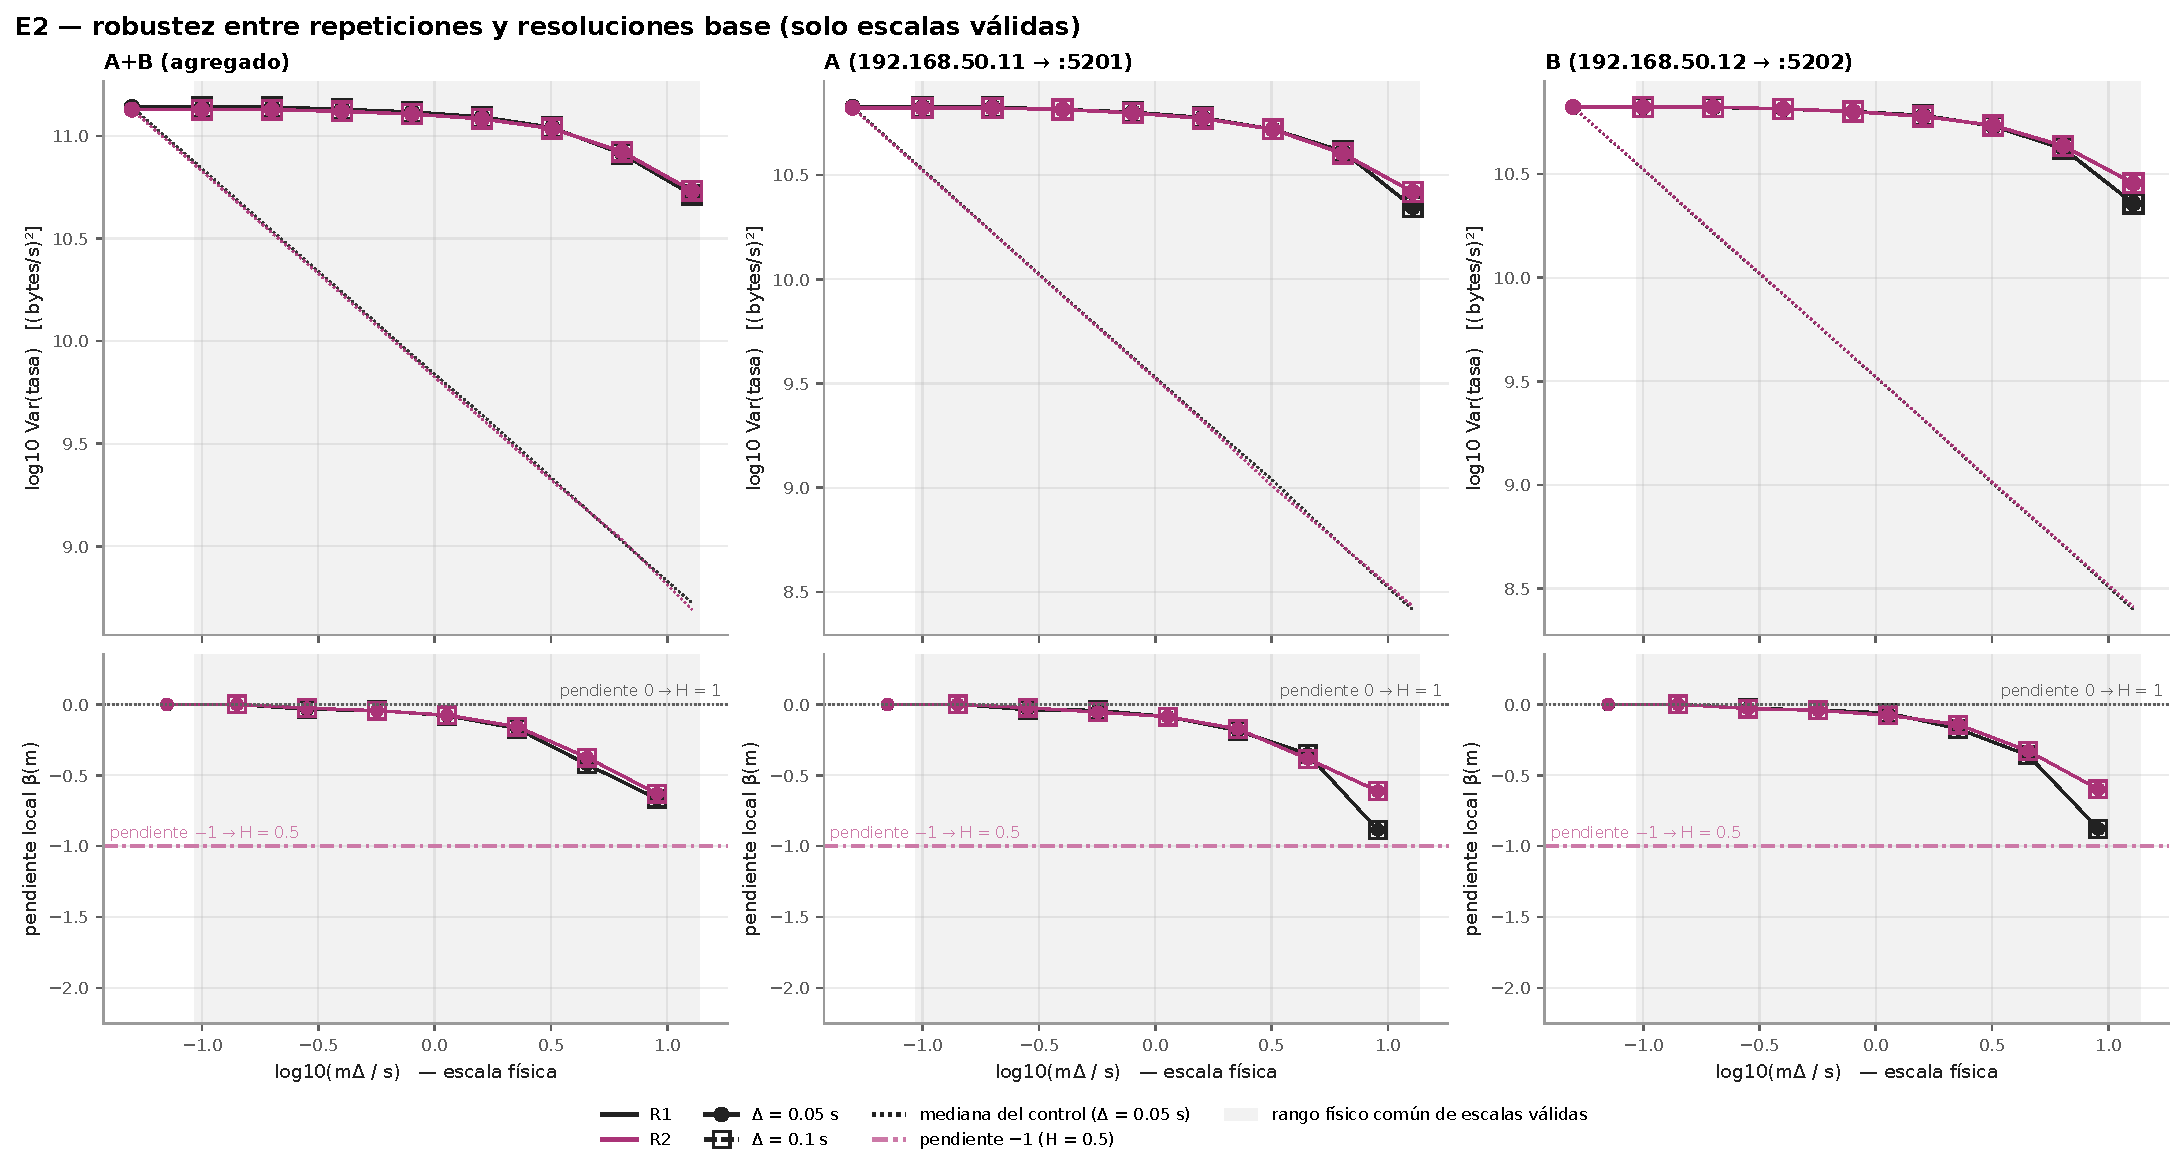
\includegraphics[width=0.85\textwidth]{robust_E2.pdf}
\caption{E2: varianza de la tasa en escala física para R1/R2 y $\Delta = 0.05/0.10$~s (arriba) y pendiente local entre escalas vecinas (abajo).}
\label{fig:robust}
\end{figure*}

\section{Resultados}
La Tabla~\ref{tab:res} reúne las 16 estimaciones. Todas tienen un tramo estable y todas quedan fuera del rango del control: por debajo en E1 y por encima en E2.

\subsection{Series temporales}
En E1 (Fig.~\ref{fig:a1}) la tasa media es 4.140~Mbit/s y el coeficiente de variación (CV) cae de 0.025 a 0.0037 y a 0.0004 a 0.05, 0.4 y 3.2~s: se divide por $\sim$7 en cada agregación $\times 8$, frente a $\sqrt{8} \approx 2.8$ para datos independientes. No hay intervalos vacíos ni tendencia ($p = 0.94$). En E2 (Fig.~\ref{fig:ts}) el CV del agregado casi no baja (0.75, 0.74, 0.67) y las ráfagas y silencios persisten en las tres resoluciones; el agregado está en silencio el 28--29\,\% del tiempo, con silencios de hasta 14~s (R1) y 21~s (R2).

\subsection{Varianza agregada}
En E1 la varianza cae con pendiente local entre $-1.5$ y $-2.2$ en todas las escalas (Fig.~\ref{fig:vte1}); en la mayor escala es unas 200 veces menor que la del control. En E2 las curvas de A+B, A y B son casi planas hasta $\sim$0.4~s y se empinan después hasta $-0.6$/$-0.9$ (Fig.~\ref{fig:vte2}); en la mayor escala la varianza es unas 100 veces mayor que la del control.

\begin{figure}[!t]
\centering
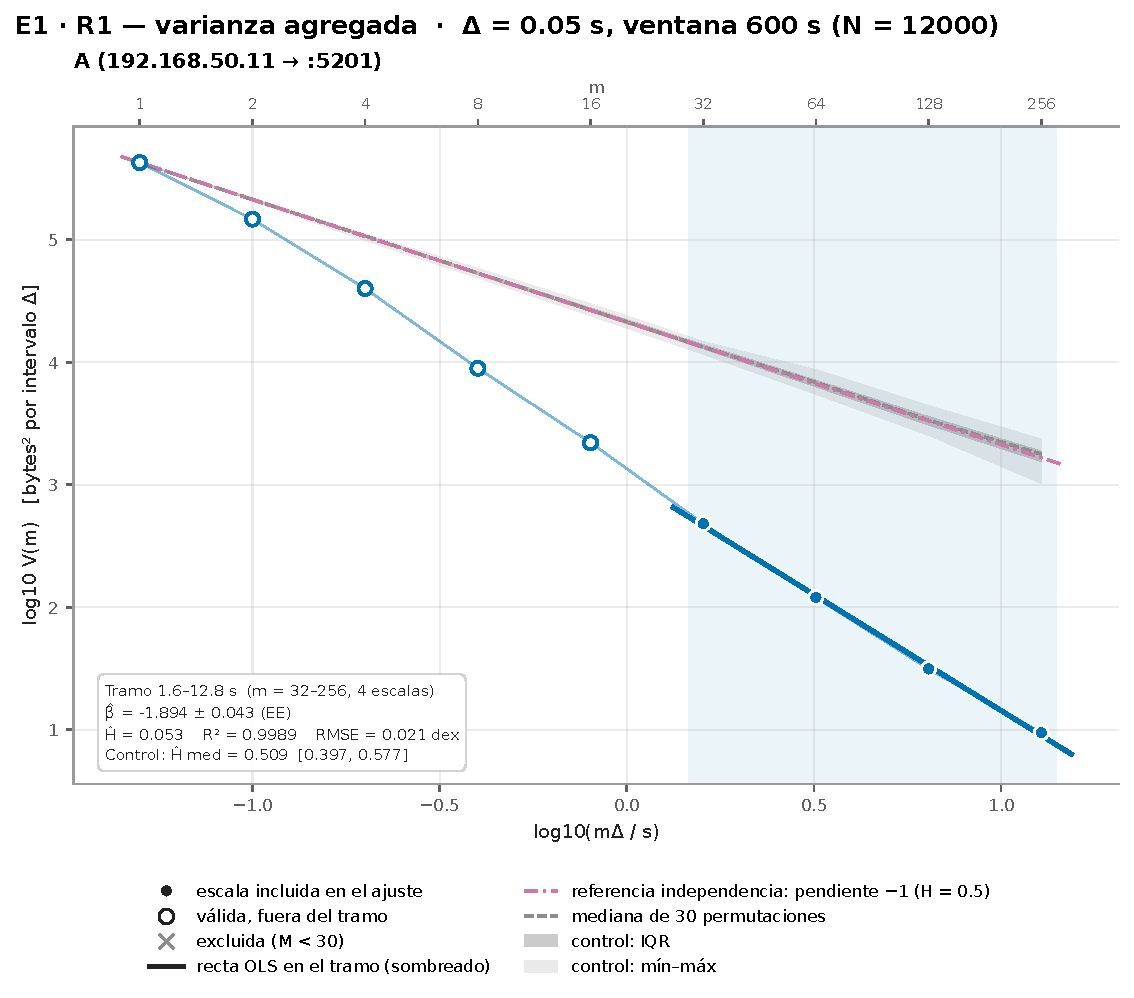
\includegraphics[width=0.88\columnwidth]{vt_E1_R1_d005.pdf}
\caption{E1\_R1: varianza agregada ($\Delta = 0.05$~s). Puntos rellenos: tramo ajustado; banda gris: 30 permutaciones; trazo-punto: pendiente $-1$ ($H = 0.5$).}
\label{fig:vte1}
\end{figure}

\subsection{Robustez}
Entre $\Delta = 0.05$ y 0.10~s, $\Hhat$ cambia como mucho 0.007: con el mismo $t_0$ los bloques de 0.10~s son uniones exactas de dos de 0.05~s y la varianza de la tasa coincide exactamente en las escalas físicas comunes. Entre repeticiones, $|\Delta\Hhat| \le 0.002$ en E2. En E1 el ajuste eligió tramos distintos (1.6--12.8~s y 0.1--0.8~s; $\Hhat = 0.053$ y 0.029), pero la pendiente local es la misma en todo el rango (Fig.~\ref{fig:robust}, Fig.~\ref{fig:a13}).

\subsection{Periodicidad}
E1 presenta líneas espectrales en 3.33, 6.67 y 10~Hz, $\sim$2.9 décadas por encima del fondo (Fig.~\ref{fig:psd}). A 416.7 datagramas/s caben 20.83 tramas por intervalo de 0.05~s, y el patrón se repite cada 6 intervalos (0.3~s = 125 tramas): es un artefacto de muestreo. En E2 no hay líneas estrechas; la potencia por debajo de 0.3~Hz supera al control en $\sim$1 década en promedio y hasta 2.3, con máximo hacia 0.04~Hz ($\sim$25~s), la escala del ciclo ON/OFF (Fig.~\ref{fig:a11}).

\begin{figure}[!t]
\centering
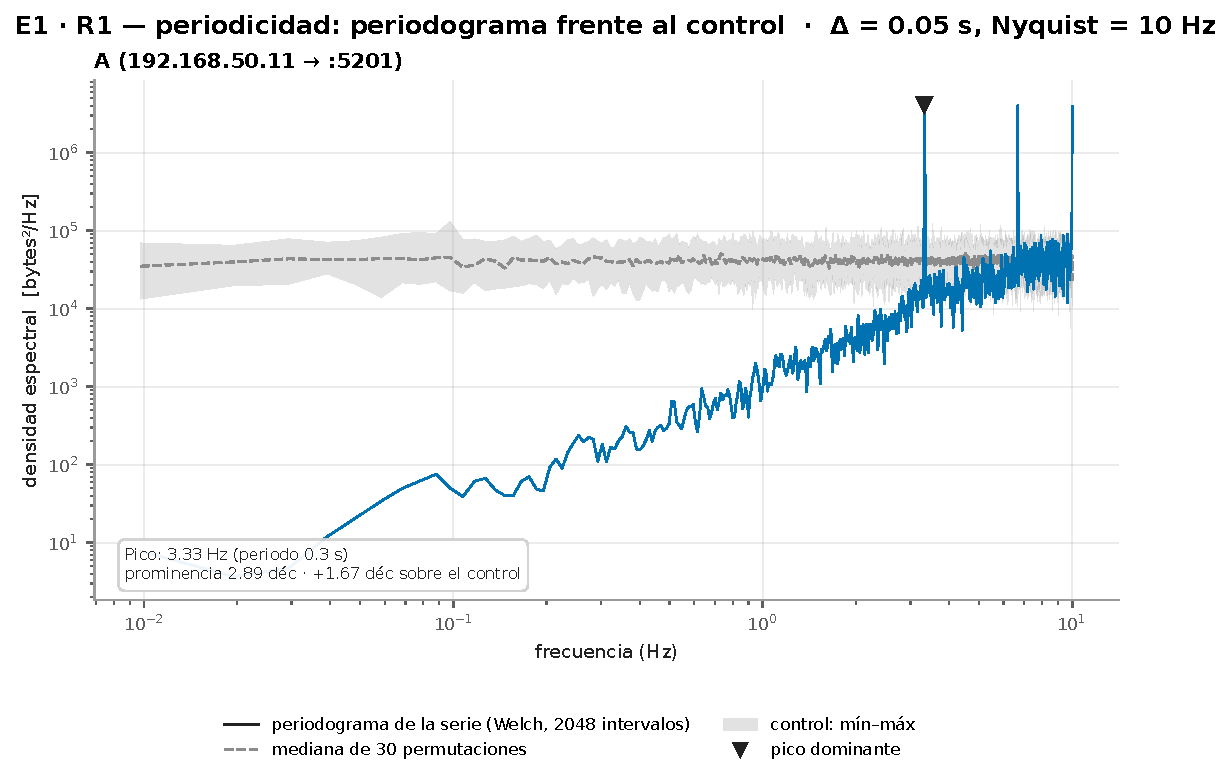
\includegraphics[width=0.92\columnwidth]{psd_E1_R1.pdf}
\caption{E1\_R1: periodograma de Welch frente a 30 permutaciones; líneas en 3.33~Hz y armónicos.}
\label{fig:psd}
\end{figure}

\begin{figure}[!t]
\centering
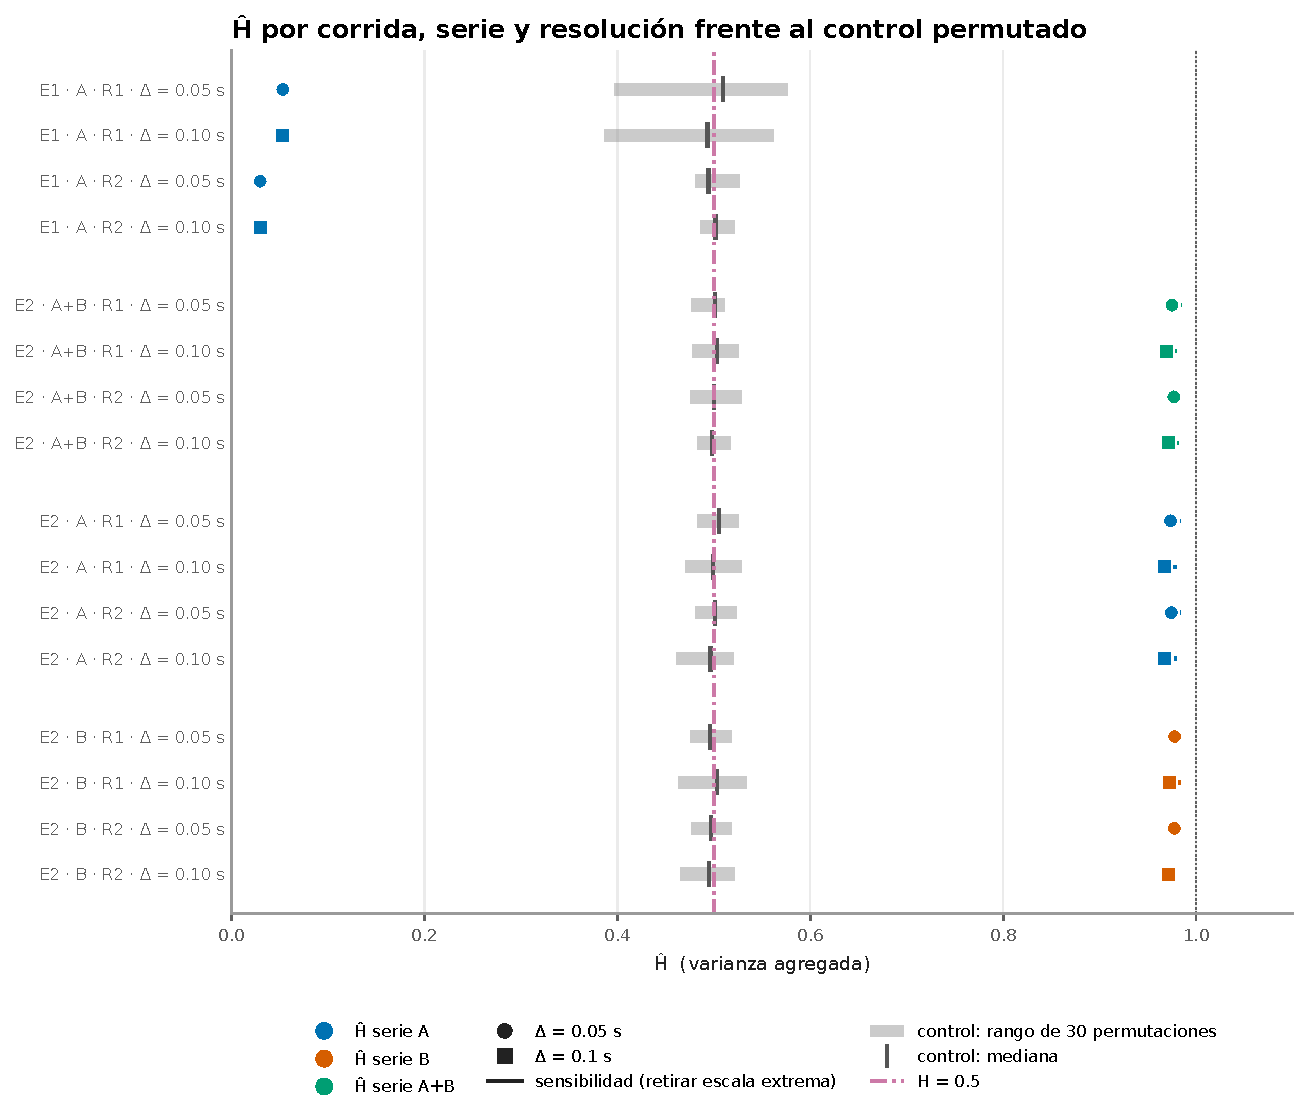
\includegraphics[width=\columnwidth]{H_summary.pdf}
\caption{Las 16 estimaciones de $\Hhat$ frente al rango y la mediana del control.}
\label{fig:hsum}
\end{figure}

\section{Discusión}
\subsection{Variabilidad y escalas de ráfagas}
En E1 la agregación suaviza la tasa más rápido que el azar: cada intervalo lleva entre 12 y 29 tramas, casi siempre 20 o 21. En E2 las ráfagas persisten hasta escalas comparables a la duración de los periodos ON y OFF, es decir, de segundos.

\subsection{Agregado frente a fuentes individuales}
A+B es más estable que cada fuente (CV 0.75 frente a 1.0--1.1) porque los periodos activos de una llenan en parte los silencios de la otra (solo A: 24--26\,\%; solo B: 22--25\,\%; ambas: 22--24\,\%; silencio: 28--29\,\%). Sin embargo, la forma de $V(m)$ y $\Hhat$ coinciden (0.974--0.978): sumar dos fuentes ON/OFF independientes con duraciones acotadas no crea un escalamiento nuevo, a diferencia de la superposición de muchas fuentes de alta variabilidad~\cite{willinger97}. Las ráfagas observadas coinciden con el cronograma el 99.7\,\% del tiempo; la diferencia es el arranque de iperf3 ($\sim$0.1~s por ráfaga).

\subsection{Comparación con el control y estabilidad}
Hay dependencia temporal en ambos escenarios, de signo opuesto: antipersistencia en E1 y persistencia en E2 (Fig.~\ref{fig:hsum}). La conclusión es estable frente a la resolución y entre repeticiones.

\subsection{Autosimilitud y limitaciones}
E2 cumple el criterio formal en 0.05--3.2~s (tramo estable, fuera del control, sensibilidad pequeña), pero la pendiente local cambia de forma continua en lugar de mantenerse: corresponde a un proceso ON/OFF cuya correlación se pierde por encima de la duración de los periodos. Lo que más limita la conclusión es la ventana de 600~s con $M_m \ge 30$, que deja la escala máxima en 12.8~s, menor que los periodos más largos (20~s). Además, la red es emulada: sin switch físico ni tráfico cruzado, E1 probablemente es más regular que en equipos reales. Los IC95\,\% del archivo de resultados suponen residuos independientes y son solo indicativos.

\section{Conclusiones}
\begin{itemize}
\item \textbf{E1 no muestra autosimilitud}: es antipersistente ($\bhat \approx -1.9$ en 0.1--12.8~s), como corresponde a un emisor de tasa constante.
\item \textbf{E2 no es compatible con autosimilitud de segundo orden en banda amplia}: presenta una persistencia aparente ($\Hhat \approx 0.97$) en 0.05--3.2~s, reproducible, explicada por el cronograma ON/OFF de 1--20~s.
\item El control por permutación, la pendiente local y el periodograma fueron decisivos para no confundir dependencia temporal con autosimilitud.
\end{itemize}

\section*{Disponibilidad de datos y código}
Capturas PCAP, CSV, código (análisis, interfaz gráfica y script de emulación), figuras y tablas: \url{https://github.com/CamiloCometa/autosimilitud-lan}. Con la semilla fija los resultados son reproducibles.

\begin{thebibliography}{9}
\bibitem{leland94} W. E. Leland, M. S. Taqqu, W. Willinger, and D. V. Wilson, ``On the self-similar nature of Ethernet traffic (extended version),'' \emph{IEEE/ACM Trans. Netw.}, vol.~2, no.~1, pp.~1--15, Feb. 1994.
\bibitem{willinger97} W. Willinger, M. S. Taqqu, R. Sherman, and D. V. Wilson, ``Self-similarity through high-variability: Statistical analysis of Ethernet LAN traffic at the source level,'' \emph{IEEE/ACM Trans. Netw.}, vol.~5, no.~1, pp.~71--86, Feb. 1997.
\bibitem{beran94} J. Beran, \emph{Statistics for Long-Memory Processes}. New York, NY, USA: Chapman \& Hall, 1994.
\bibitem{taqqu95} M. S. Taqqu, V. Teverovsky, and W. Willinger, ``Estimators for long-range dependence: An empirical study,'' \emph{Fractals}, vol.~3, no.~4, pp.~785--798, 1995.
\bibitem{lantz10} B. Lantz, B. Heller, and N. McKeown, ``A network in a laptop: Rapid prototyping for software-defined networks,'' in \emph{Proc. 9th ACM SIGCOMM Workshop Hot Topics Netw. (HotNets)}, 2010, pp.~1--6.
\bibitem{iperf} ESnet, ``iperf3: Invoking iperf3.'' [Online]. Available: \url{https://software.es.net/iperf/invoking.html}
\bibitem{tshark} Wireshark Foundation, ``tshark(1) manual page.'' [Online]. Available: \url{https://www.wireshark.org/docs/man-pages/tshark.html}
\end{thebibliography}

\clearpage
\onecolumn
\appendices
\section{Figuras complementarias}
Se incluyen las 13 figuras restantes del análisis, con su lectura.

\begin{figure}[!htbp]
\centering
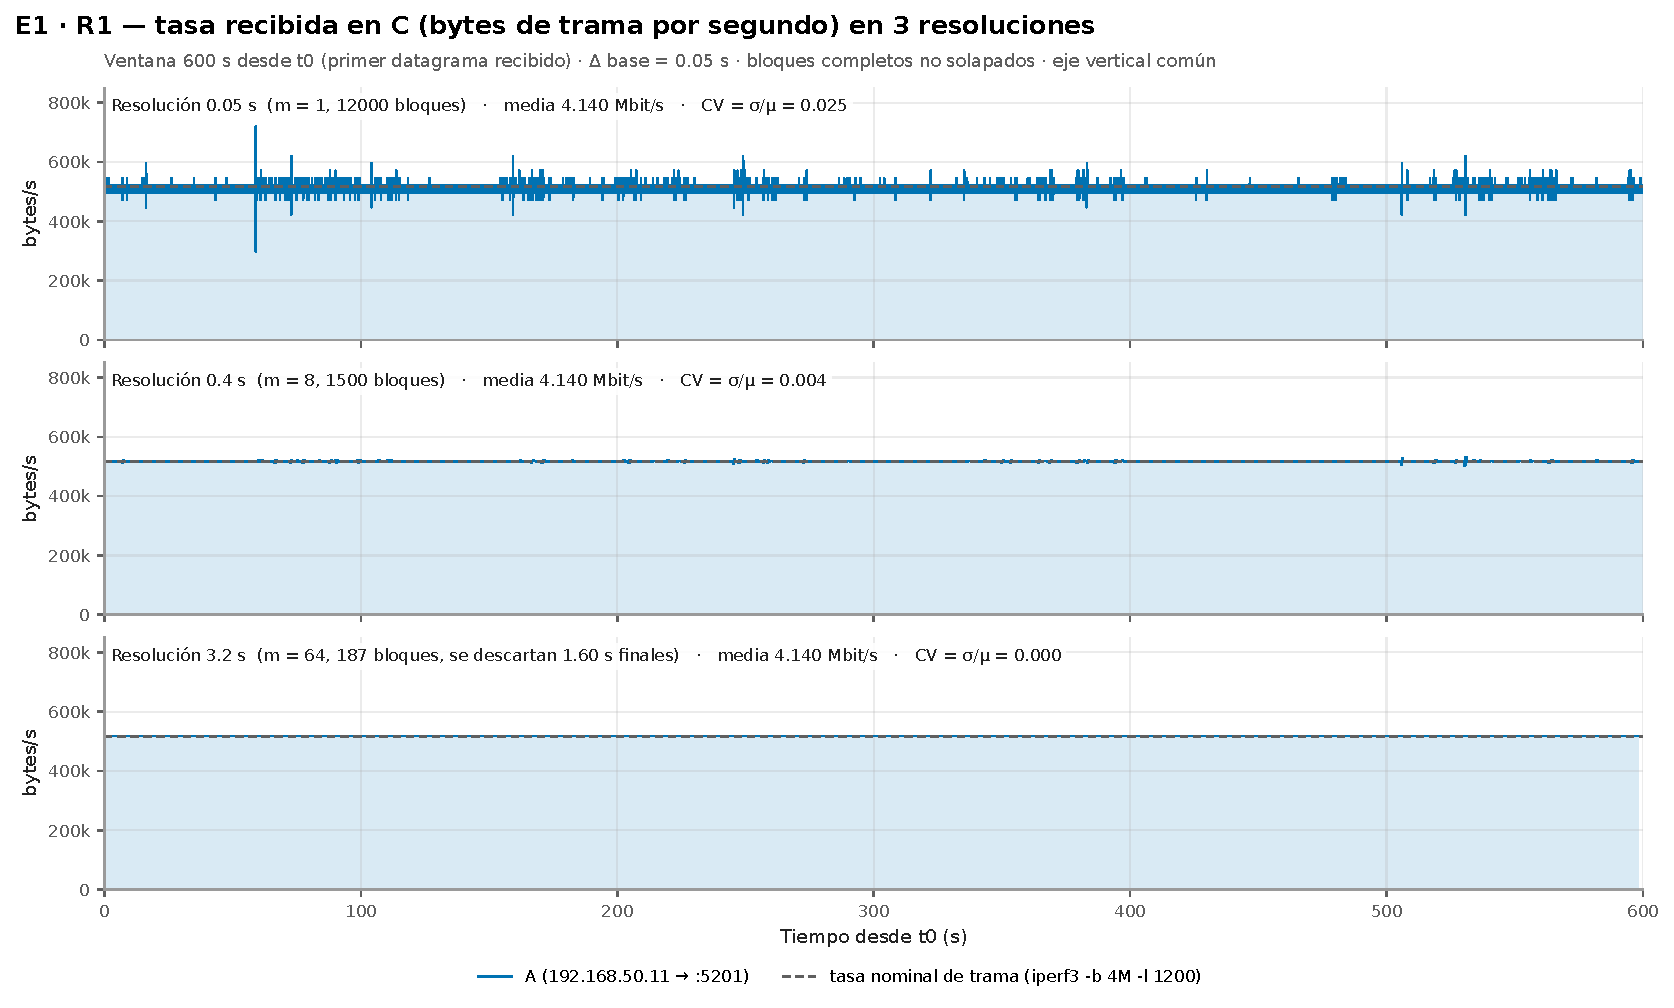
\includegraphics[width=0.82\textwidth]{ts_E1_R1.pdf}
\caption{E1\_R1: tasa en tres resoluciones. Media 4.140~Mbit/s (línea discontinua: tasa nominal de trama, 517.5~kB/s). CV 0.025, 0.0037 y 0.0004; máximo 720, 531 y 518~kB/s; sin intervalos vacíos ni tendencia.}
\label{fig:a1}
\vspace{8pt}
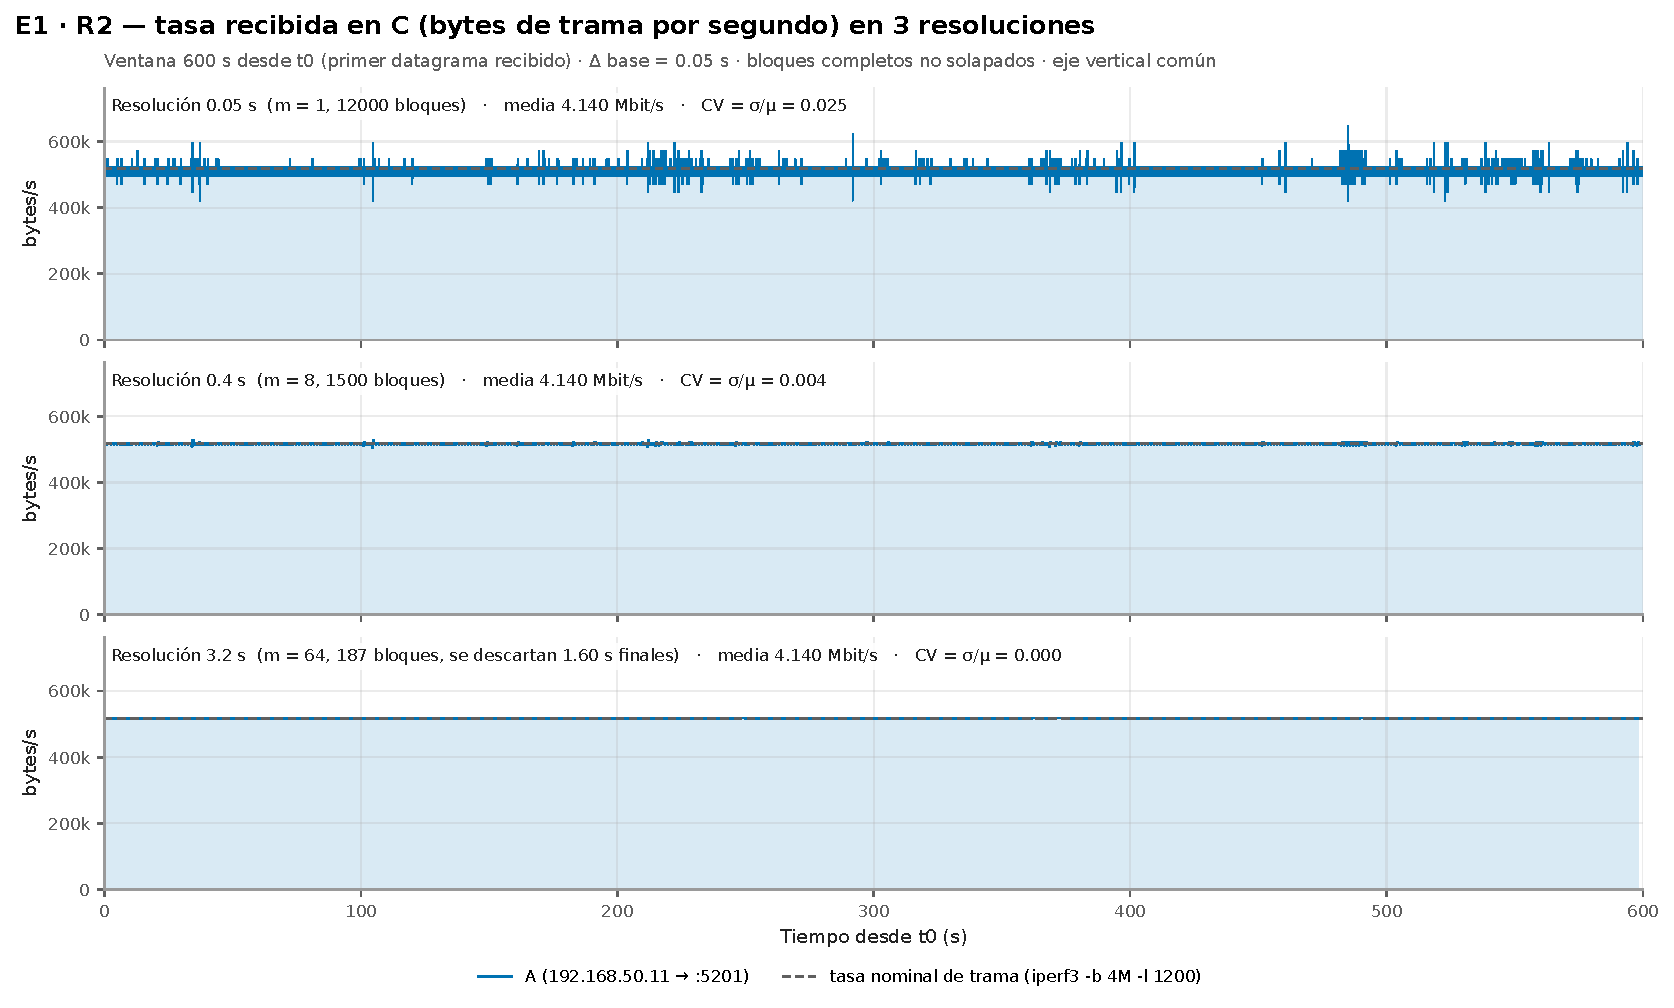
\includegraphics[width=0.82\textwidth]{ts_E1_R2.pdf}
\caption{E1\_R2: igual que R1 (4.140~Mbit/s; CV 0.025, 0.0036 y 0.0004; sin intervalos vacíos). La regularidad es propia del emisor.}
\label{fig:a2}
\end{figure}

\begin{figure}[!htbp]
\centering
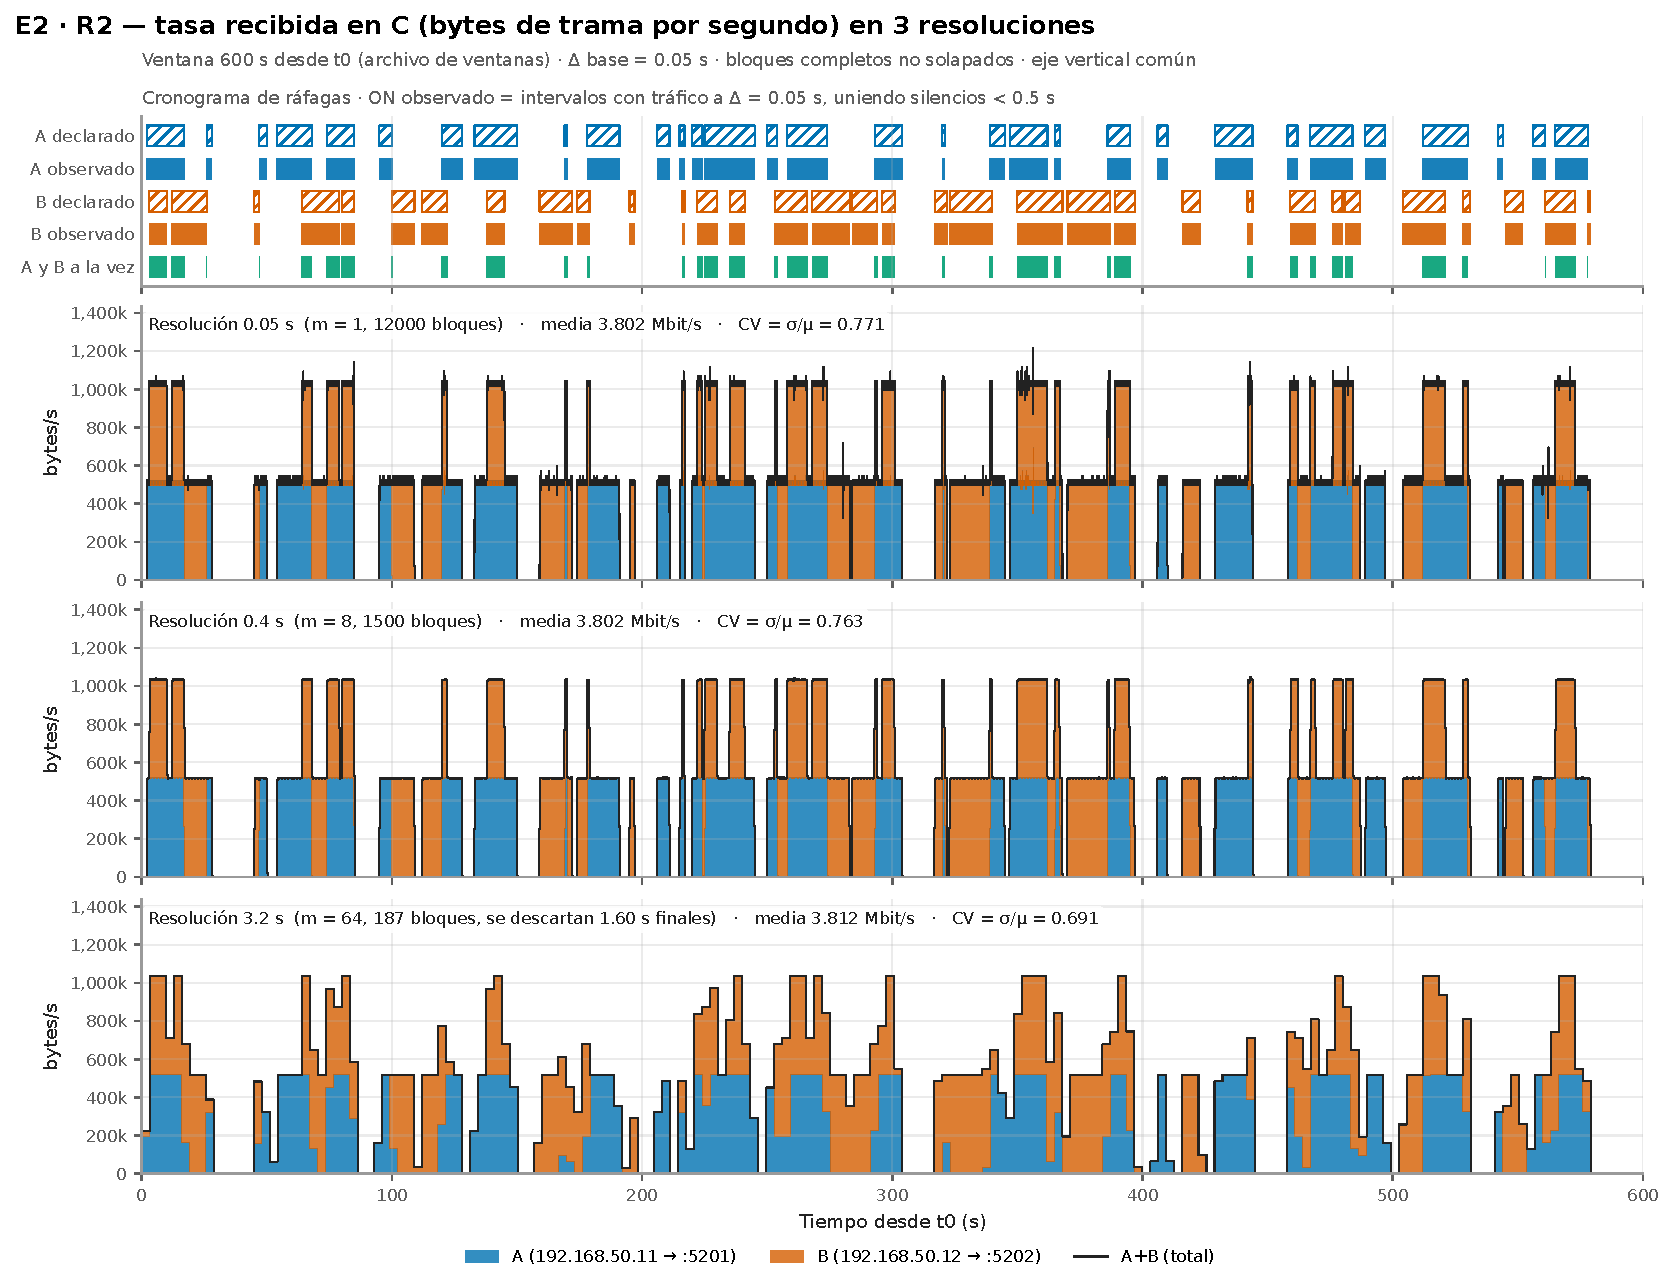
\includegraphics[width=0.9\textwidth]{ts_E2_R2.pdf}
\caption{E2\_R2: A+B promedia 3.80~Mbit/s con CV 0.77, 0.76 y 0.69. Solo A 24\,\%, solo B 25\,\%, ambos 22\,\%, silencio 29\,\%; silencio más largo 21~s; concordancia con el cronograma 99.7\,\%.}
\label{fig:a3}
\end{figure}

\begin{figure}[!htbp]
\centering
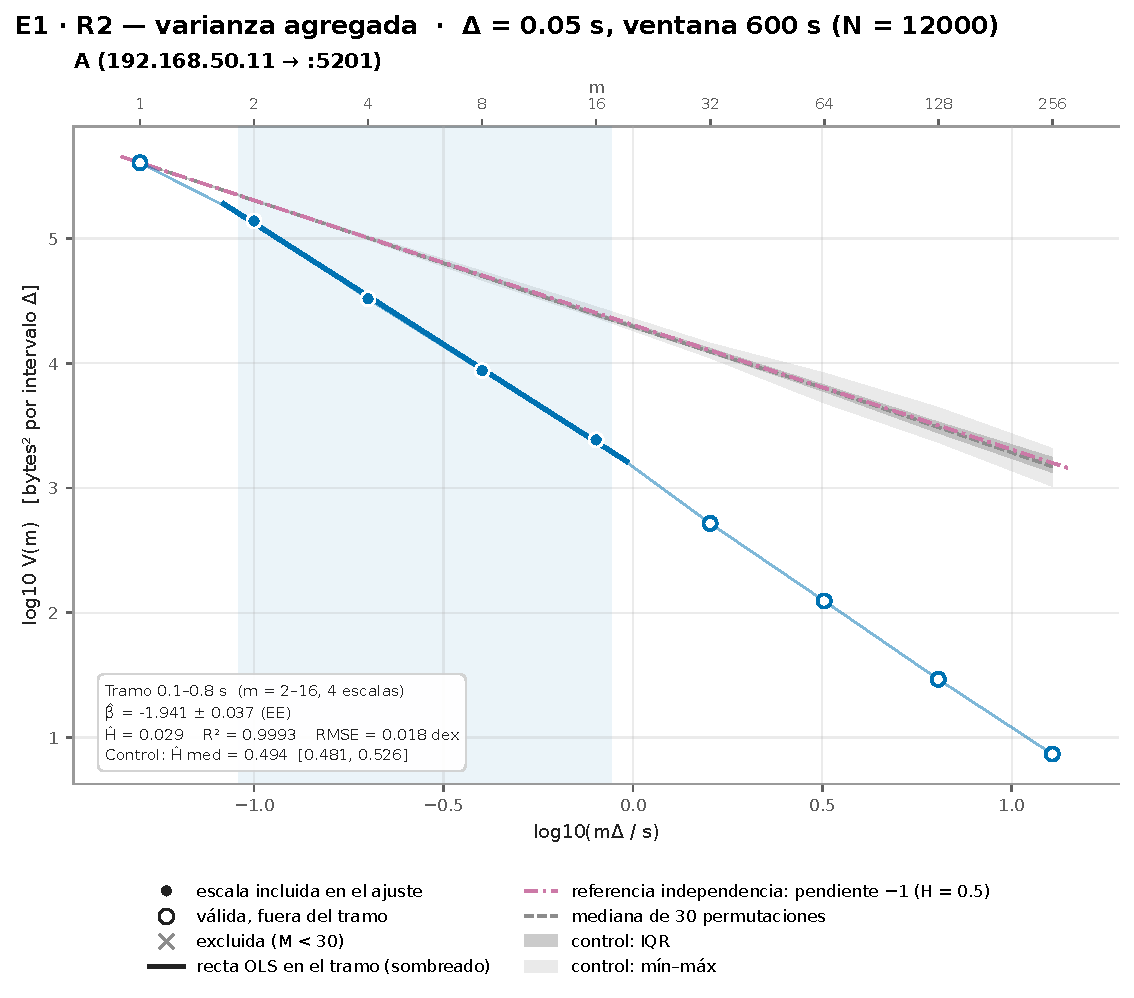
\includegraphics[width=0.5\textwidth]{vt_E1_R2_d005.pdf}
\caption{E1\_R2, $\Delta = 0.05$~s: tramo 0.1--0.8~s, $\bhat = -1.94$, $\Hhat = 0.029$, $R^2 = 0.999$. Pendiente local entre $-1.55$ y $-2.23$ en toda la curva; en la mayor escala la varianza es $\sim$200 veces menor que la del control.}
\label{fig:a4}
\vspace{8pt}
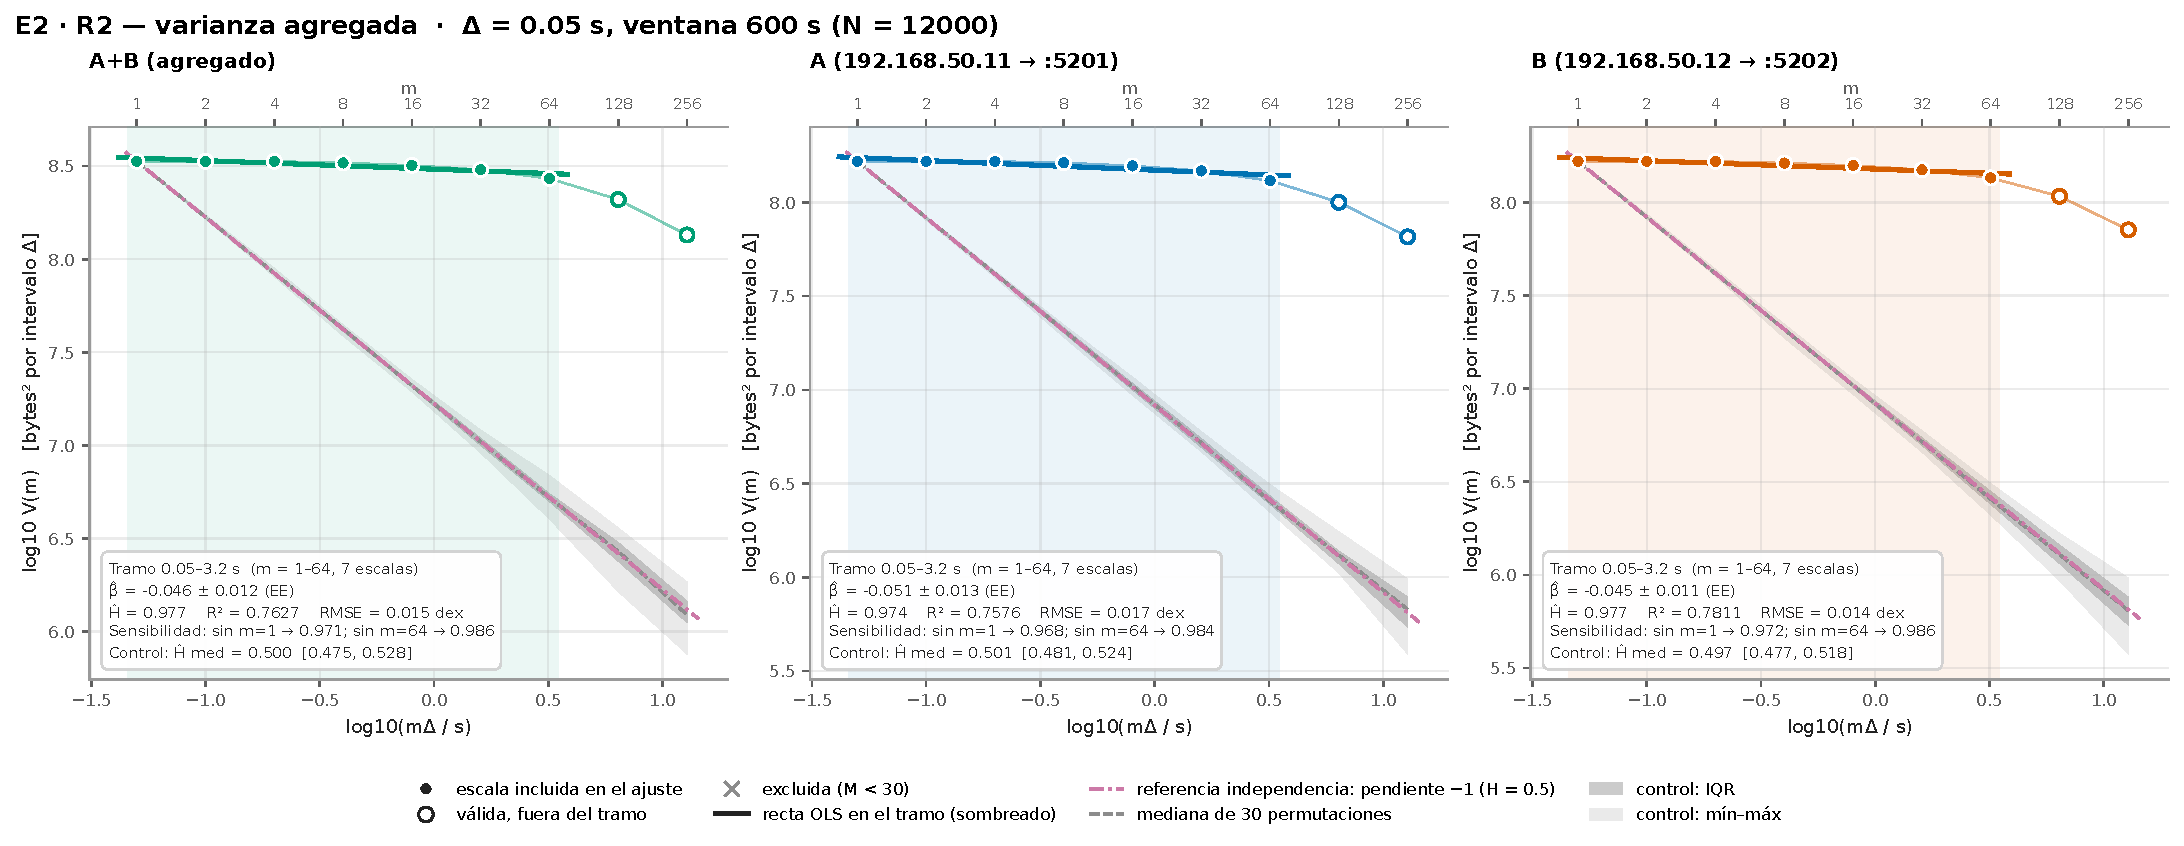
\includegraphics[width=0.95\textwidth]{vt_E2_R2_d005.pdf}
\caption{E2\_R2, $\Delta = 0.05$~s: $\Hhat = 0.974$--$0.977$ en 0.05--3.2~s; sensibilidad $< 0.01$; en la mayor escala la varianza es $\sim$100 veces mayor que la del control. Por encima de 3.2~s la curva se empina hasta $-0.6$.}
\label{fig:a5}
\end{figure}

\begin{figure}[!htbp]
\centering
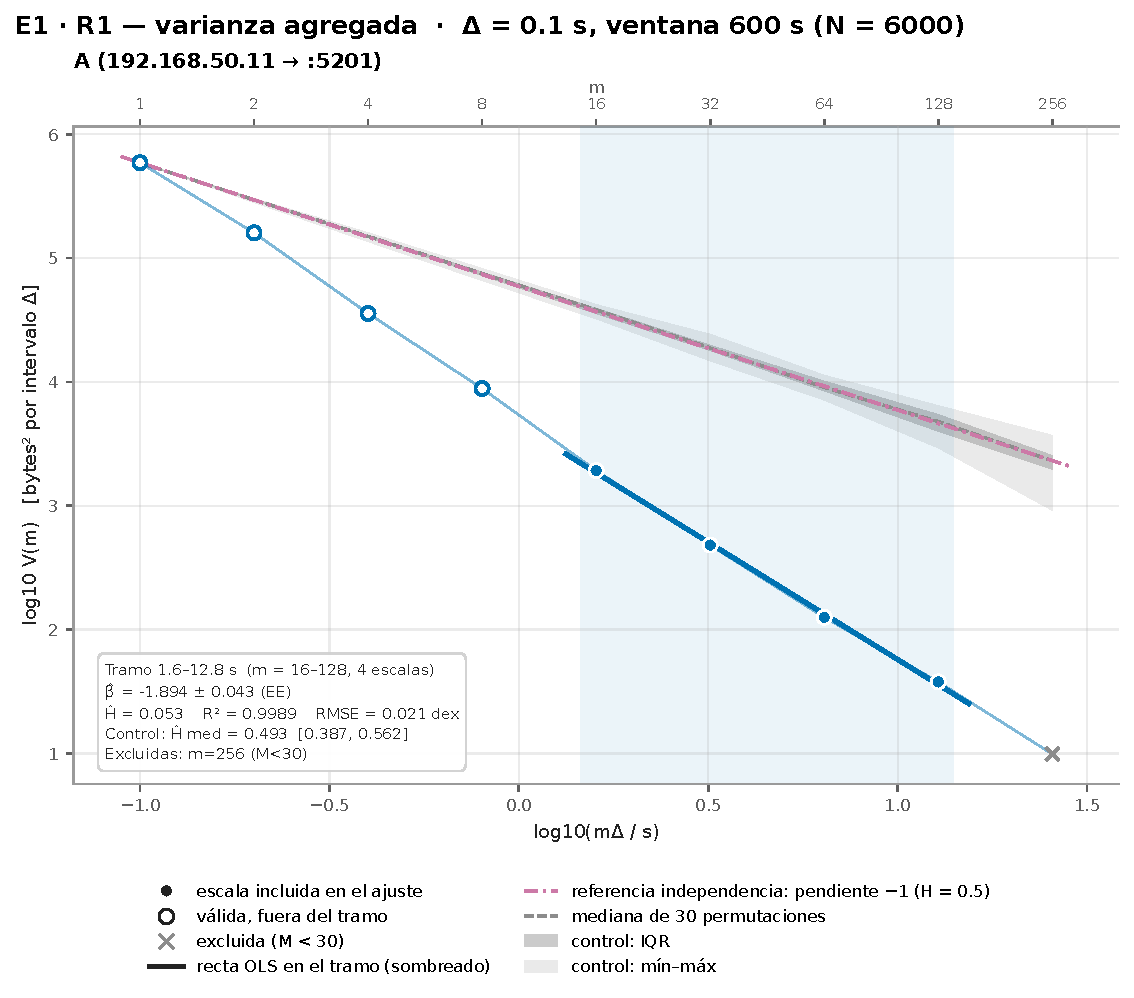
\includegraphics[width=0.48\textwidth]{vt_E1_R1_d010.pdf}\hfill
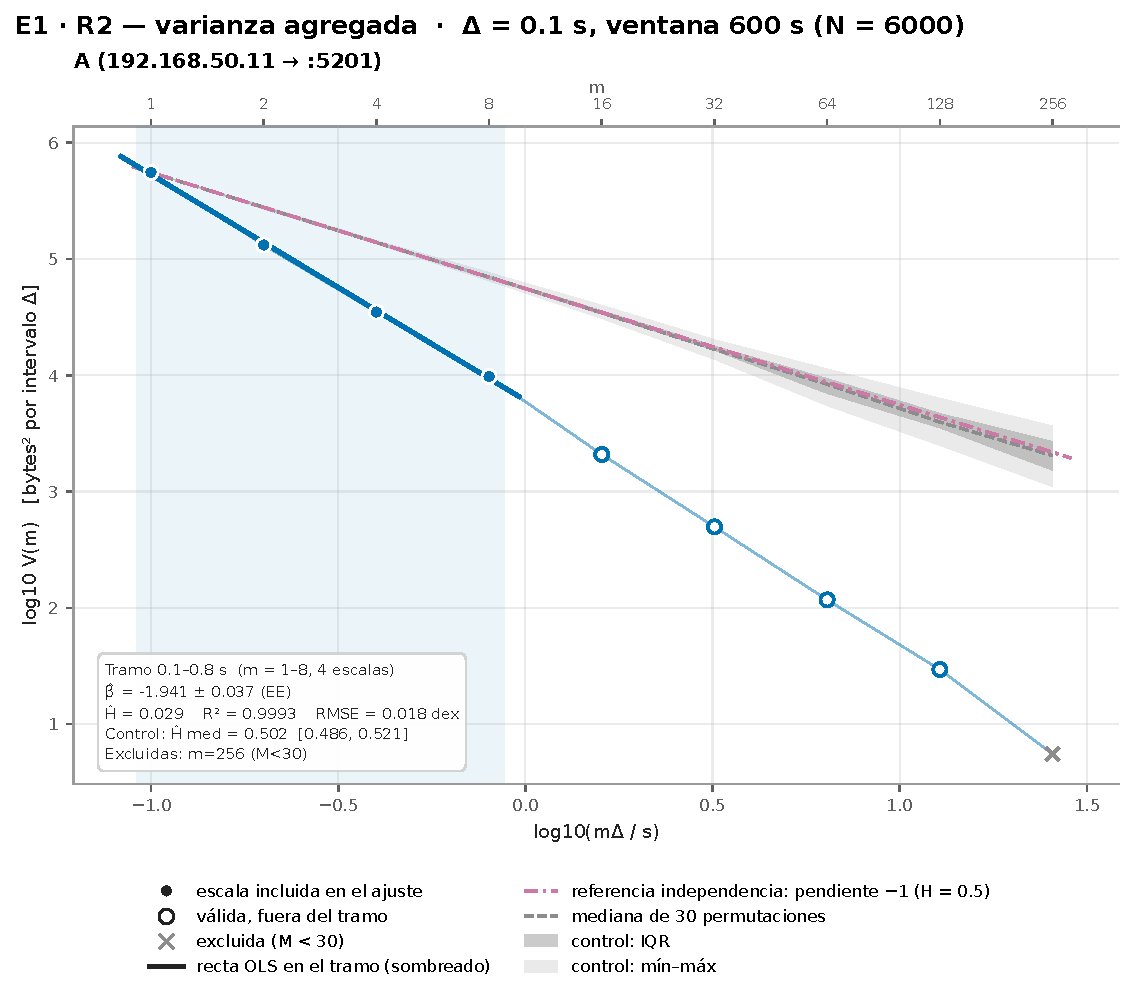
\includegraphics[width=0.48\textwidth]{vt_E1_R2_d010.pdf}
\caption{E1 con $\Delta = 0.10$~s: R1 (izq., $\Hhat = 0.053$) y R2 (der., $\Hhat = 0.029$), idénticos a $\Delta = 0.05$~s; $m = 256$ excluida ($M = 23$).}
\label{fig:a6}
\vspace{8pt}
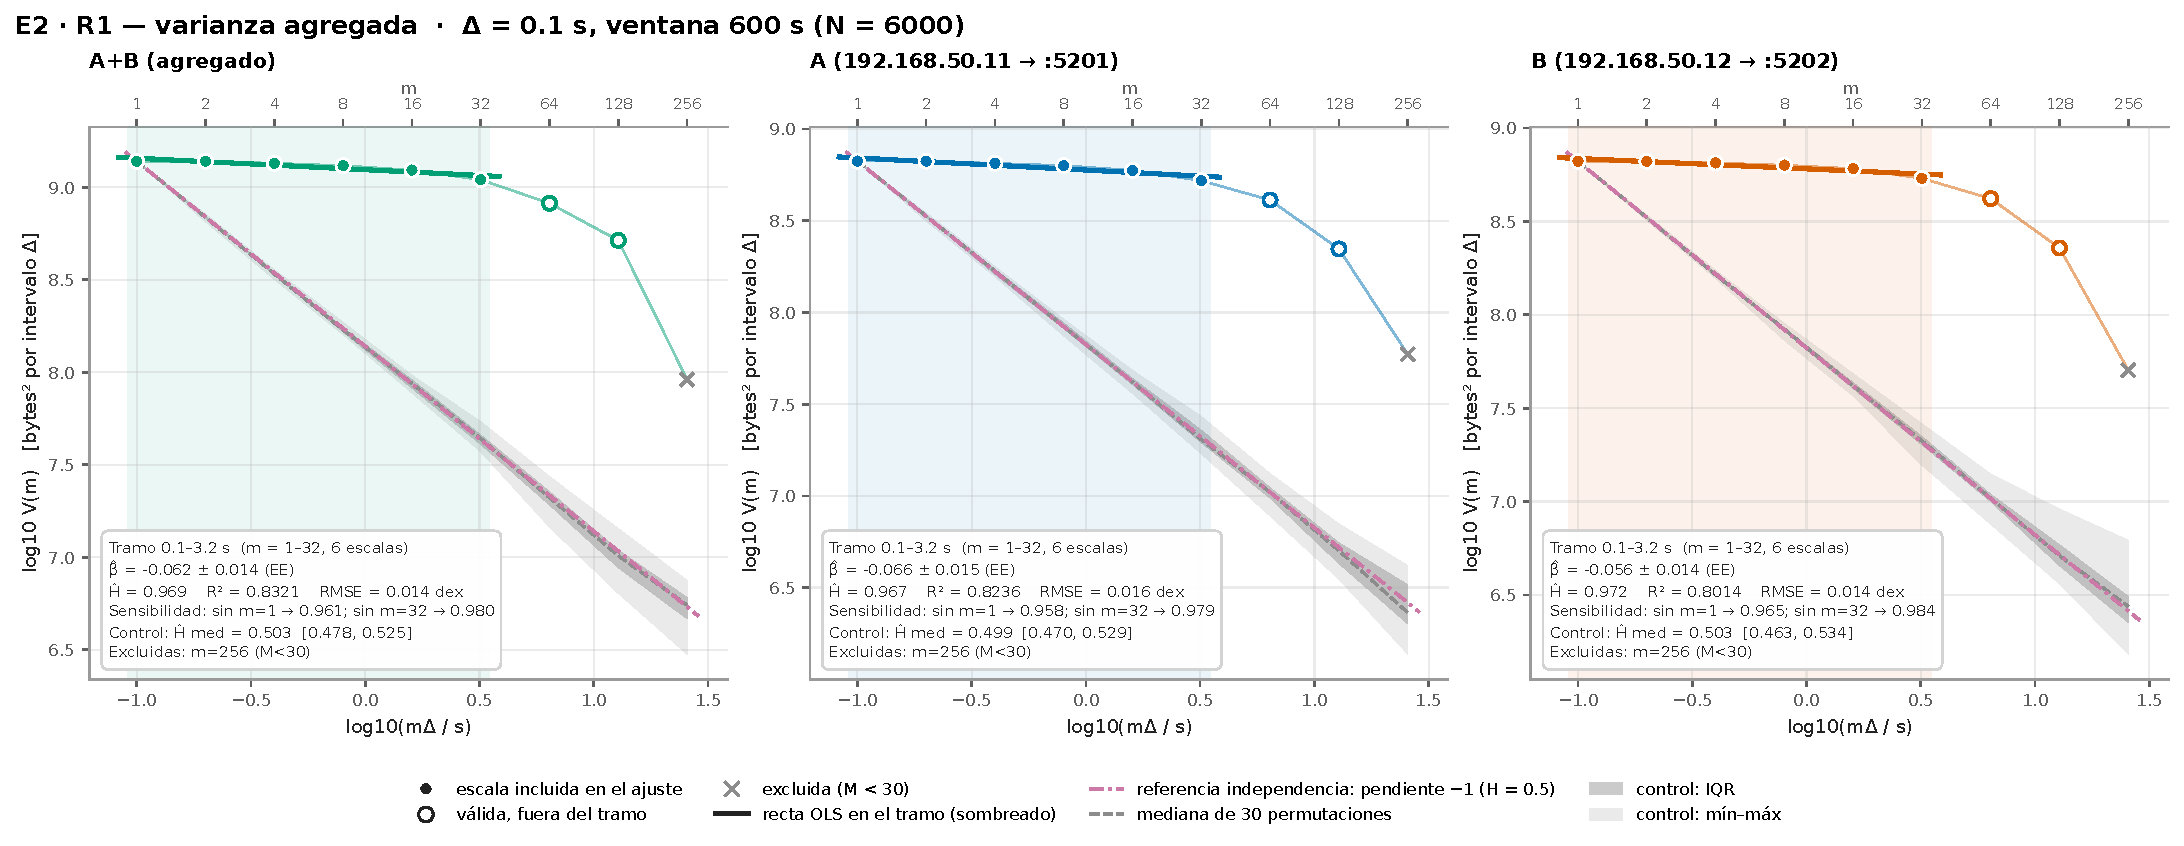
\includegraphics[width=0.95\textwidth]{vt_E2_R1_d010.pdf}
\caption{E2\_R1, $\Delta = 0.10$~s: $\Hhat = 0.969$ (A+B), 0.967 (A), 0.972 (B); 0.006 menos que con 0.05~s por perder la escala más fina, que es plana.}
\label{fig:a8}
\end{figure}

\begin{figure}[!htbp]
\centering
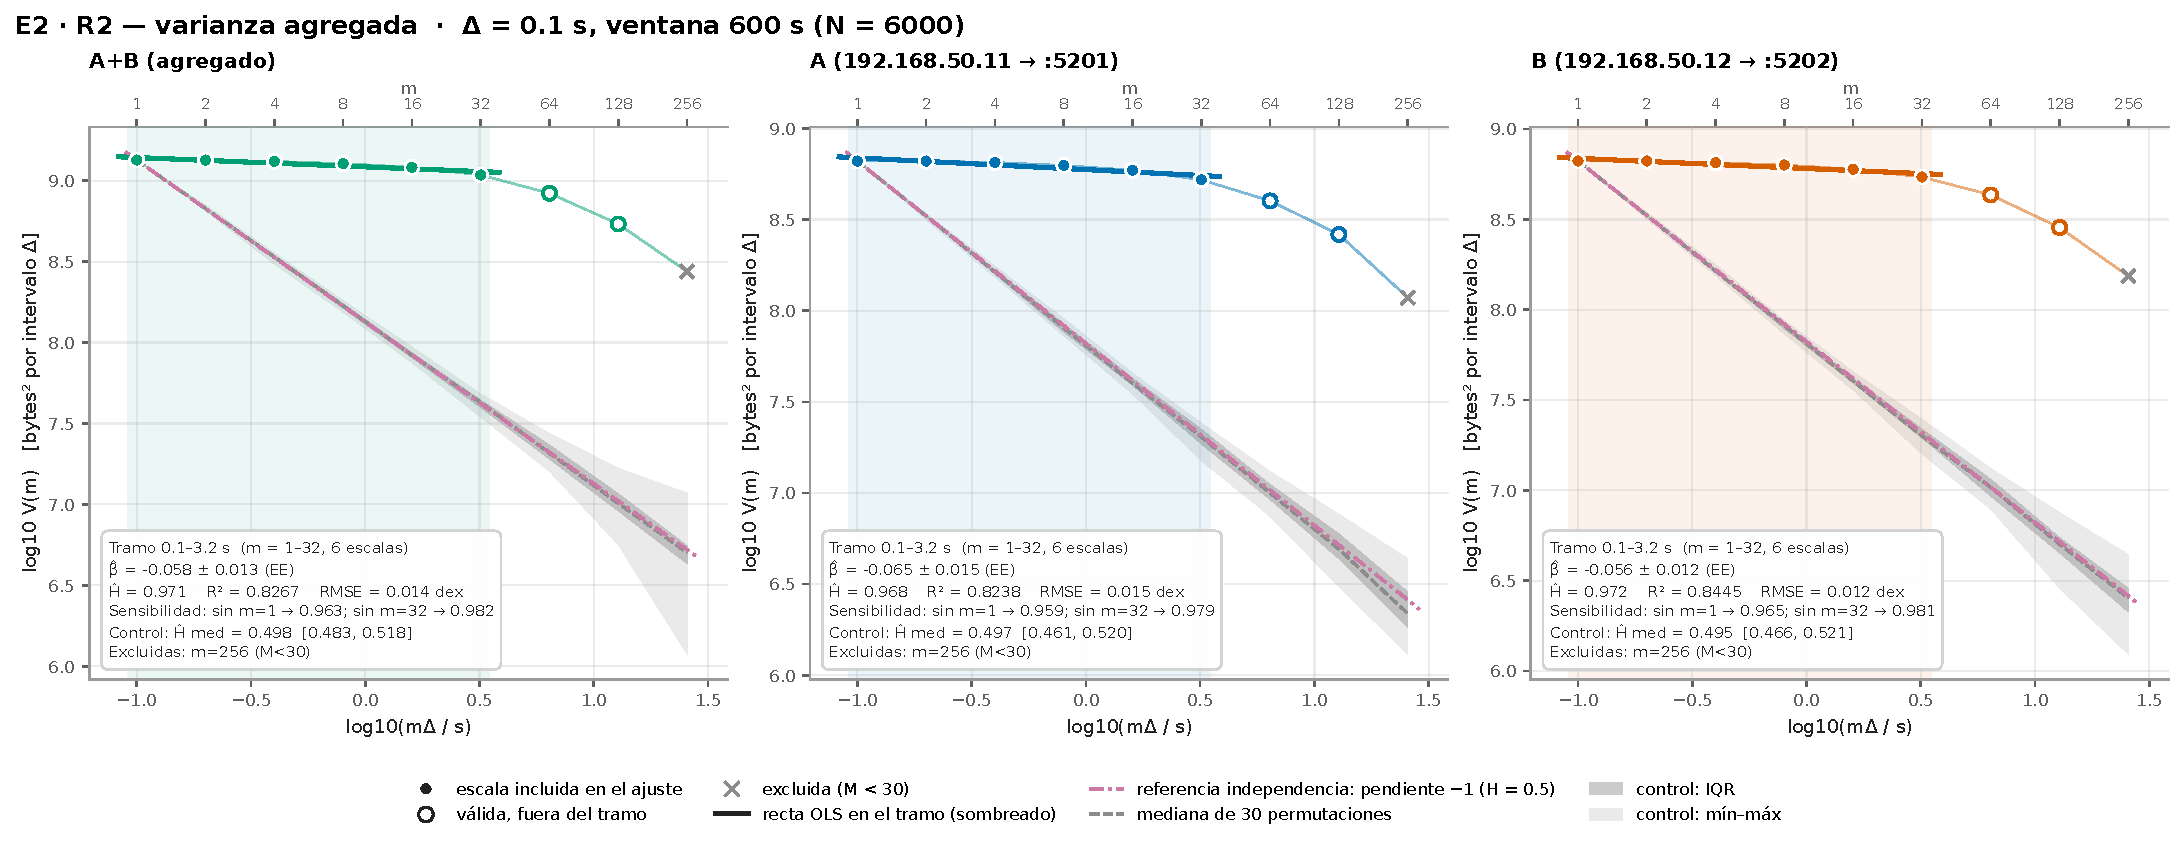
\includegraphics[width=0.95\textwidth]{vt_E2_R2_d010.pdf}
\caption{E2\_R2, $\Delta = 0.10$~s: $\Hhat = 0.971$ (A+B), 0.968 (A), 0.972 (B); el cambio de resolución mueve $\Hhat$ menos de 0.01.}
\label{fig:a9}
\vspace{8pt}
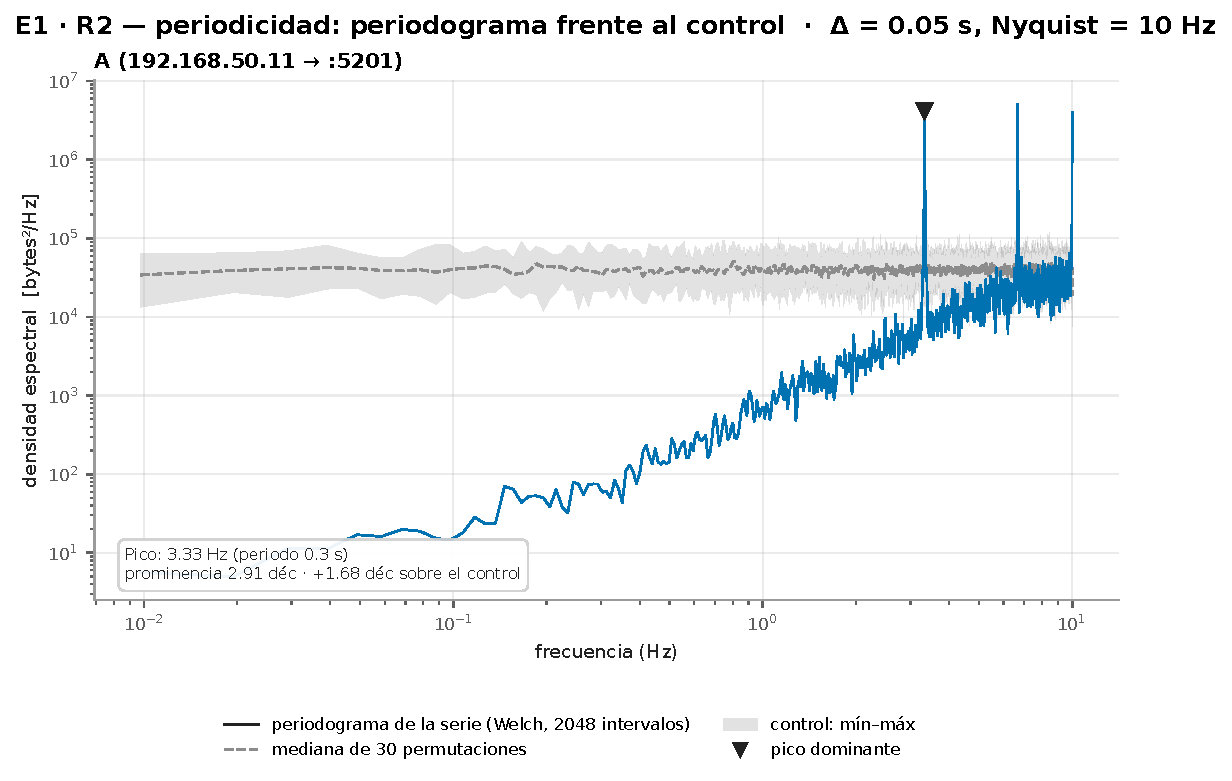
\includegraphics[width=0.55\textwidth]{psd_E1_R2.pdf}
\caption{E1\_R2: mismas líneas que R1 (3.33~Hz y armónicos; prominencia 2.9 décadas, 1.7 sobre el máximo del control). Por debajo de 1~Hz la densidad queda bajo el control y crece con la frecuencia: firma antipersistente.}
\label{fig:a10}
\end{figure}

\begin{figure}[!htbp]
\centering
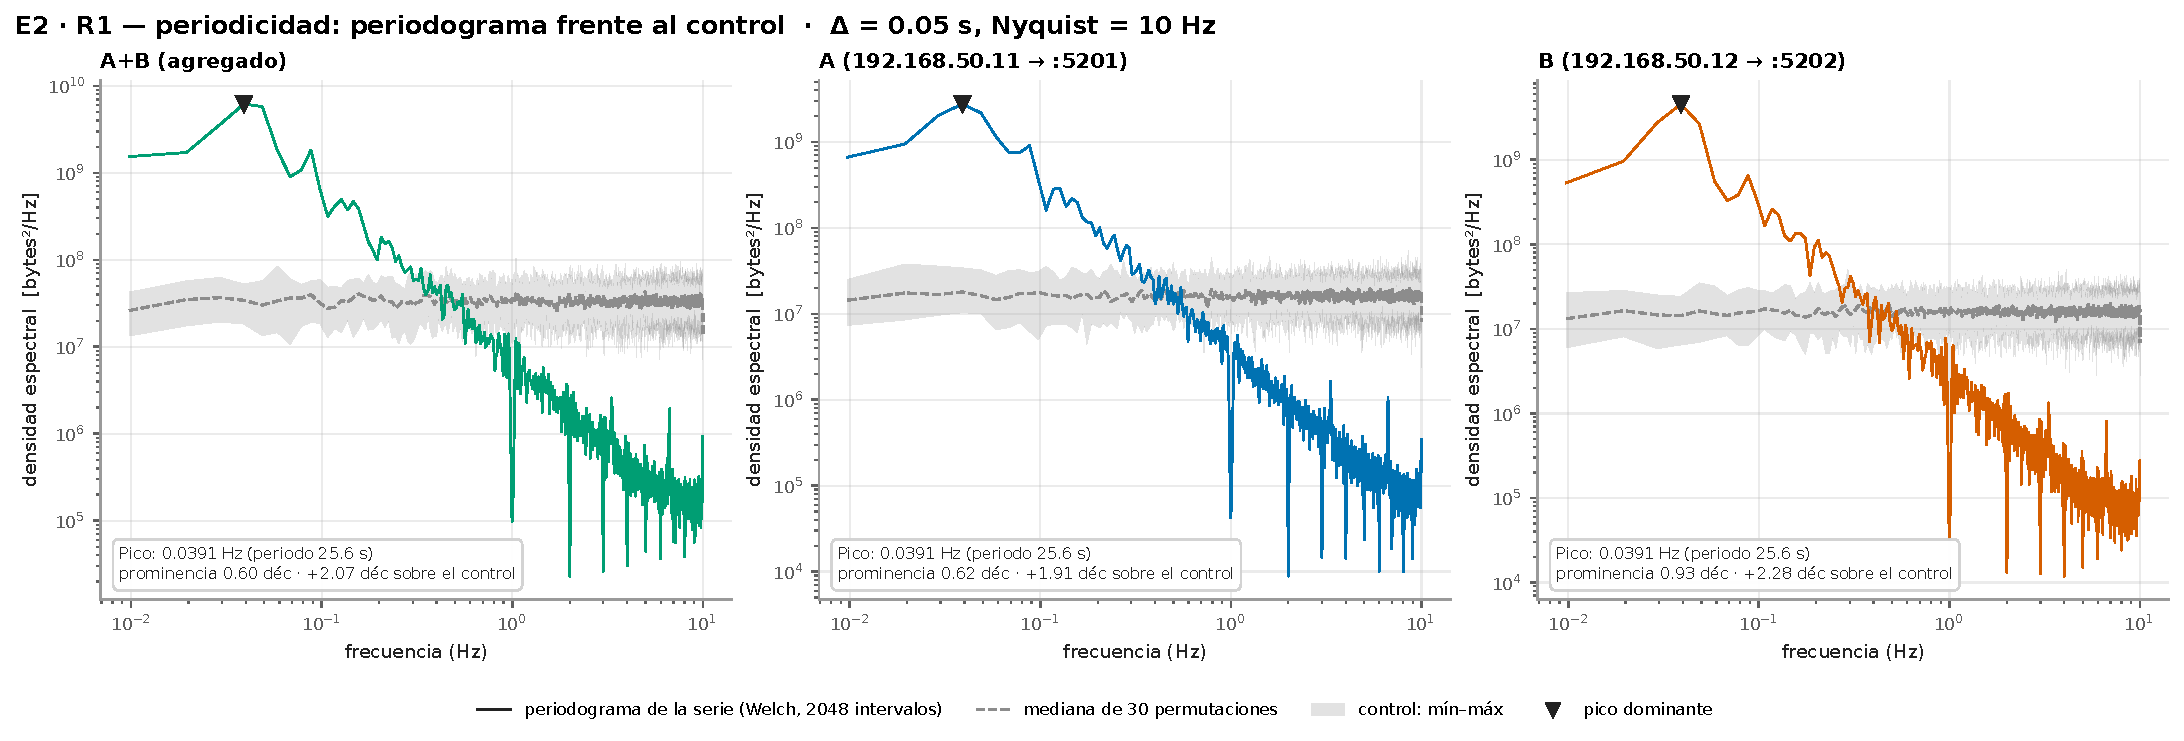
\includegraphics[width=\textwidth]{psd_E2_R1.pdf}
\caption{E2\_R1: por debajo de $\sim$0.3~Hz la potencia supera al control en $\sim$1 década en promedio y hasta 2.3, con máximo en 0.039~Hz ($\sim$25.6~s). Es una joroba ancha, no una línea: la escala de los ciclos ON/OFF ($\sim$21~s en promedio).}
\label{fig:a11}
\vspace{8pt}
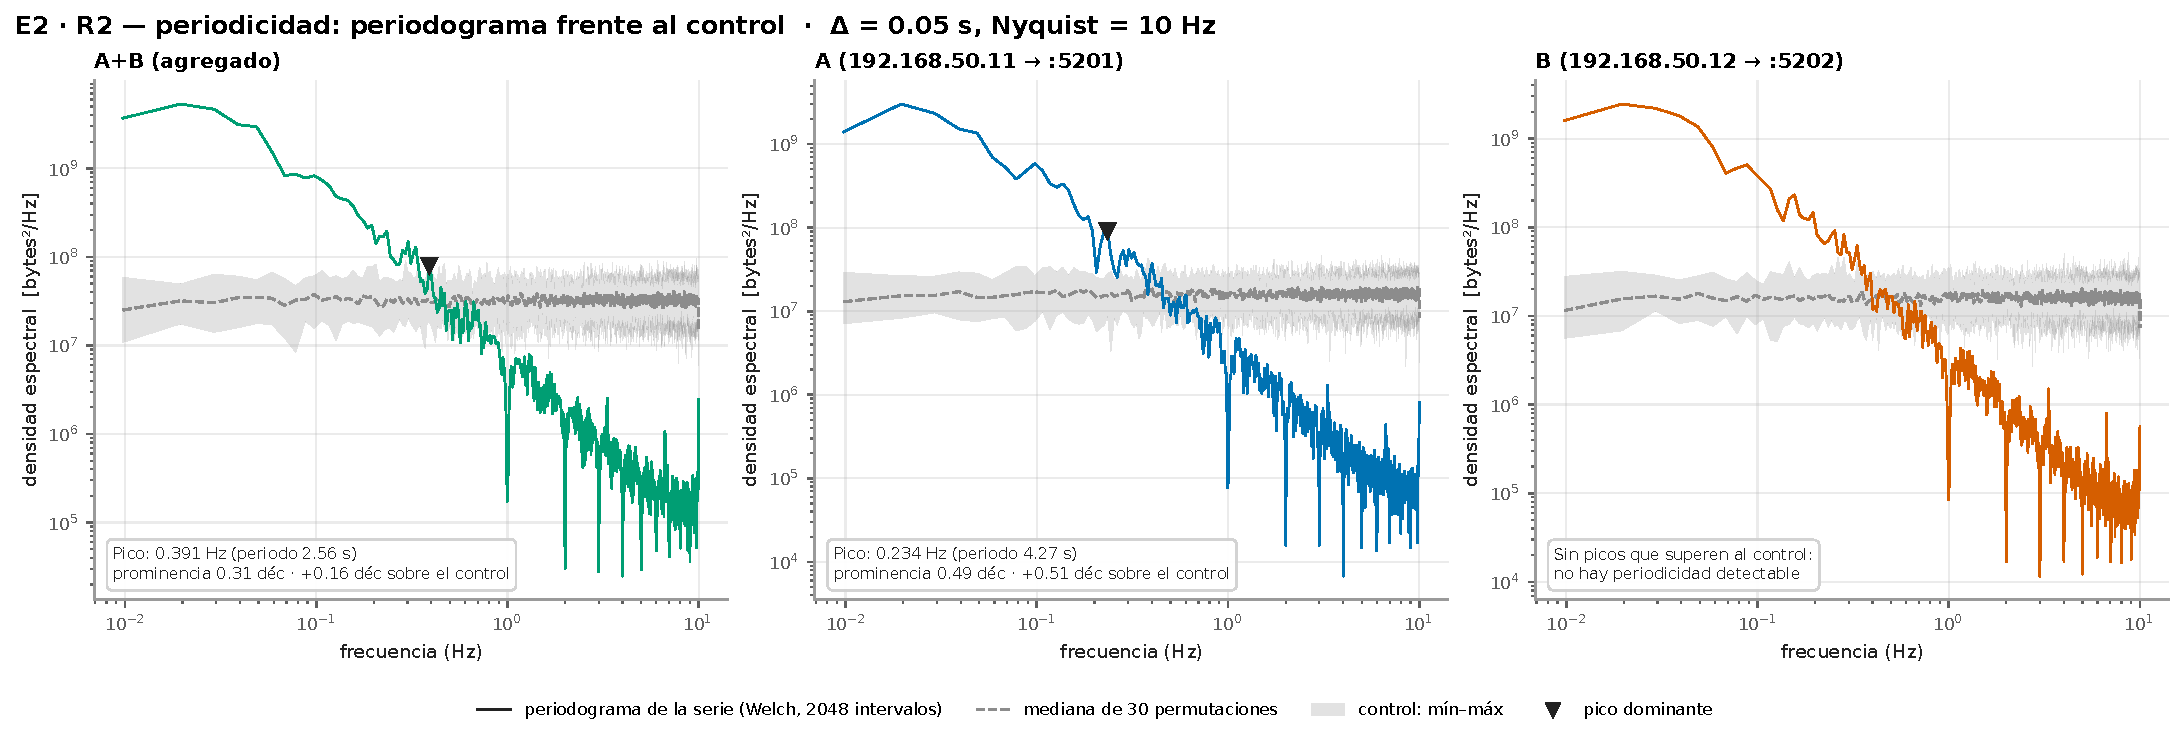
\includegraphics[width=\textwidth]{psd_E2_R2.pdf}
\caption{E2\_R2: mismo exceso en bajas frecuencias; picos débiles (0.39~Hz en A+B, 0.16 décadas sobre el control; ninguno en B). Sin periodicidad clara.}
\label{fig:a12}
\end{figure}

\begin{figure}[!htbp]
\centering
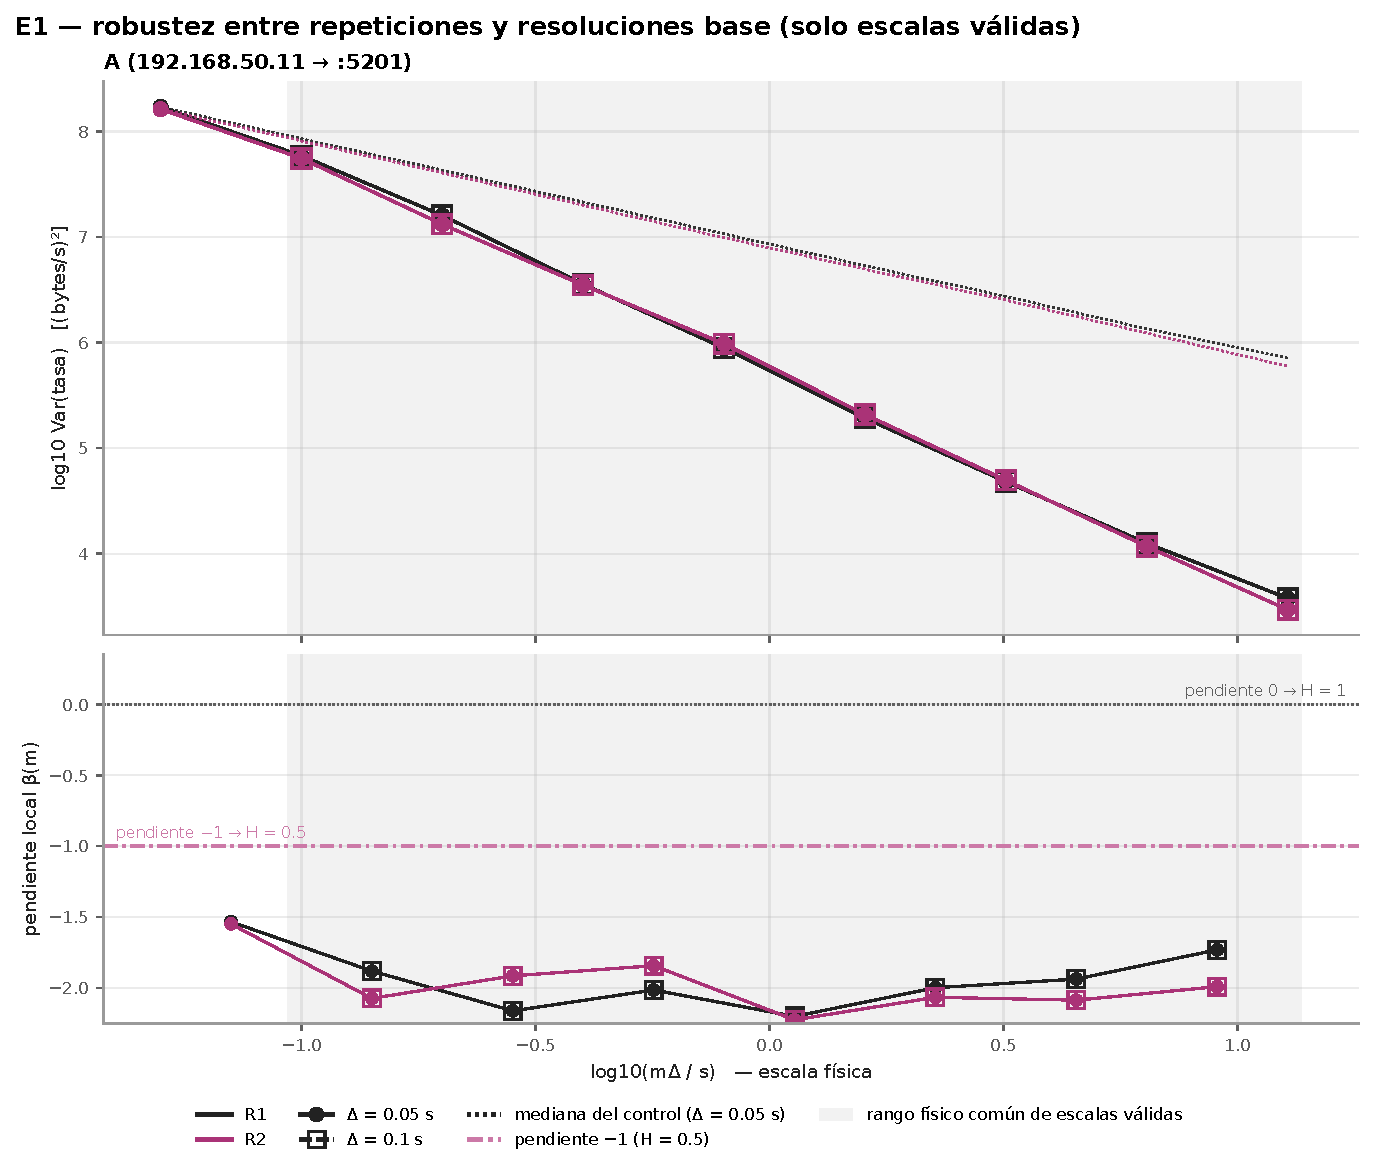
\includegraphics[width=0.75\textwidth]{robust_E1.pdf}
\caption{E1: robustez. Las curvas de R1/R2 y de las dos $\Delta$ se superponen; la pendiente local (abajo) queda entre $-1.5$ y $-2.2$ en todas las escalas, siempre por debajo de $-1$ ($H = 0.5$). La diferencia de tramo entre repeticiones no cambia la conclusión.}
\label{fig:a13}
\end{figure}

\end{document}
